\chapter{Prompt gamma detection}\label{chap::2}

\vfill

\minitoc

\newpage

\glsresetall

Ion beam therapy is rapidly emerging as a valuable cancer treatment technique and a superior alternative to photon radiotherapy for specific clinical indications. The narrow dose peak at the end of the ion range allows for targeted delivery of high dose to the tumor while sparing healthy surrounding tissues. However, since such a treatment technique is highly sensitive to dose prediction and delivery uncertainties, online range monitoring solutions are necessary. Over- and under-shooting effects potentially lead to severe damages to healthy tissues and/or treatment inefficiency, and thus have to be controlled in real-time. The research effort in this field mainly focuses on the non-invasive detection of primary by-products of beam-tissue nuclear interactions: photons from electron-positron annihilation and prompt gammas are most extensively studied for this purpose. 
The research work presented in this thesis focus on the development of gamma cameras for the detection of prompt gamma rays to tackle the challenge of real-time range monitoring during particle therapy treatments. In this chapter, after a brief introduction of the photon interaction channels in matter, the main topic of the thesis will be addressed by discussing the present developed techniques to obtain information about the ion range with prompt gamma ray detection. Finally, the state-of-the-art of gamma detectors employed for this purpose is sketched.

\section{Photon detection}


\subsection{Photon interactions in matter}

In penetrating an absorbing medium, photons may experience various interactions with the atoms of the medium, involving either the nuclei or the orbital electrons. The interactions with nuclei may be direct photon-nucleus collisions or interactions between the photon and the electrostatic field of the nucleus (pair production). On the other hand, the photon-orbital electron interactions can involve either loosely bound electrons (binding energy $E_B$ small in comparison with the photon energy $h\nu$ - $E_B \ll h\nu$) or tightly bound electrons (binding energy comparable to, or slightly smaller than the photon energy - $E_B  \lesssim h\nu$). 
All these processes are characterized by a partial or complete energy transfer of the gamma-ray photon, and two different outcomes are possible:
\begin{itemize}
\item Photon disappears (i.e. is completely absorbed) and its energy is transferred to light charged particles (electron and positrons);
\item Photon is scattered and two results are possible:
	\begin{itemize}
		\item the resulting photon has the same energy as the incident photon and no light charged particle is released in the interaction;
		\item the resulting scattered photon has a lower energy than the incident photon and the energy excess is transferred to a light charged particle (electron).
	\end{itemize}
\end{itemize}

We focus here on the interaction channels which play an important role in radiation measurements: 
\begin{itemize}
\item photoelectric absorption;
\item Compton scattering;
\item pair production.
\end{itemize}

In case the photon interacts with an absorber \myMarginnote{Photoelectric absorption} atom and completely disappears by transferring all its energy to the target, the interaction mechanism is called photoelectric absorption. In the interaction an orbital electron  is ejected with kinetic energy $E_K$ corresponding to the difference between the incident photon energy $h\nu$ and the electron binding energy $E_B$, as reported in equation~\ref{chap2::eq::energyPhotoelectron}. The ejected orbital electron is generally referred to as \enquote{photoelectron}. A schematic view of the photoelectric absorption mechanism is shown in \figurename~\ref{chap2::fig::photoel_abs}.

\begin{equation}
E_K = h\nu - E_B
\label{chap2::eq::energyPhotoelectron}
\end{equation}

\begin{figure}[!htbp]
\centering
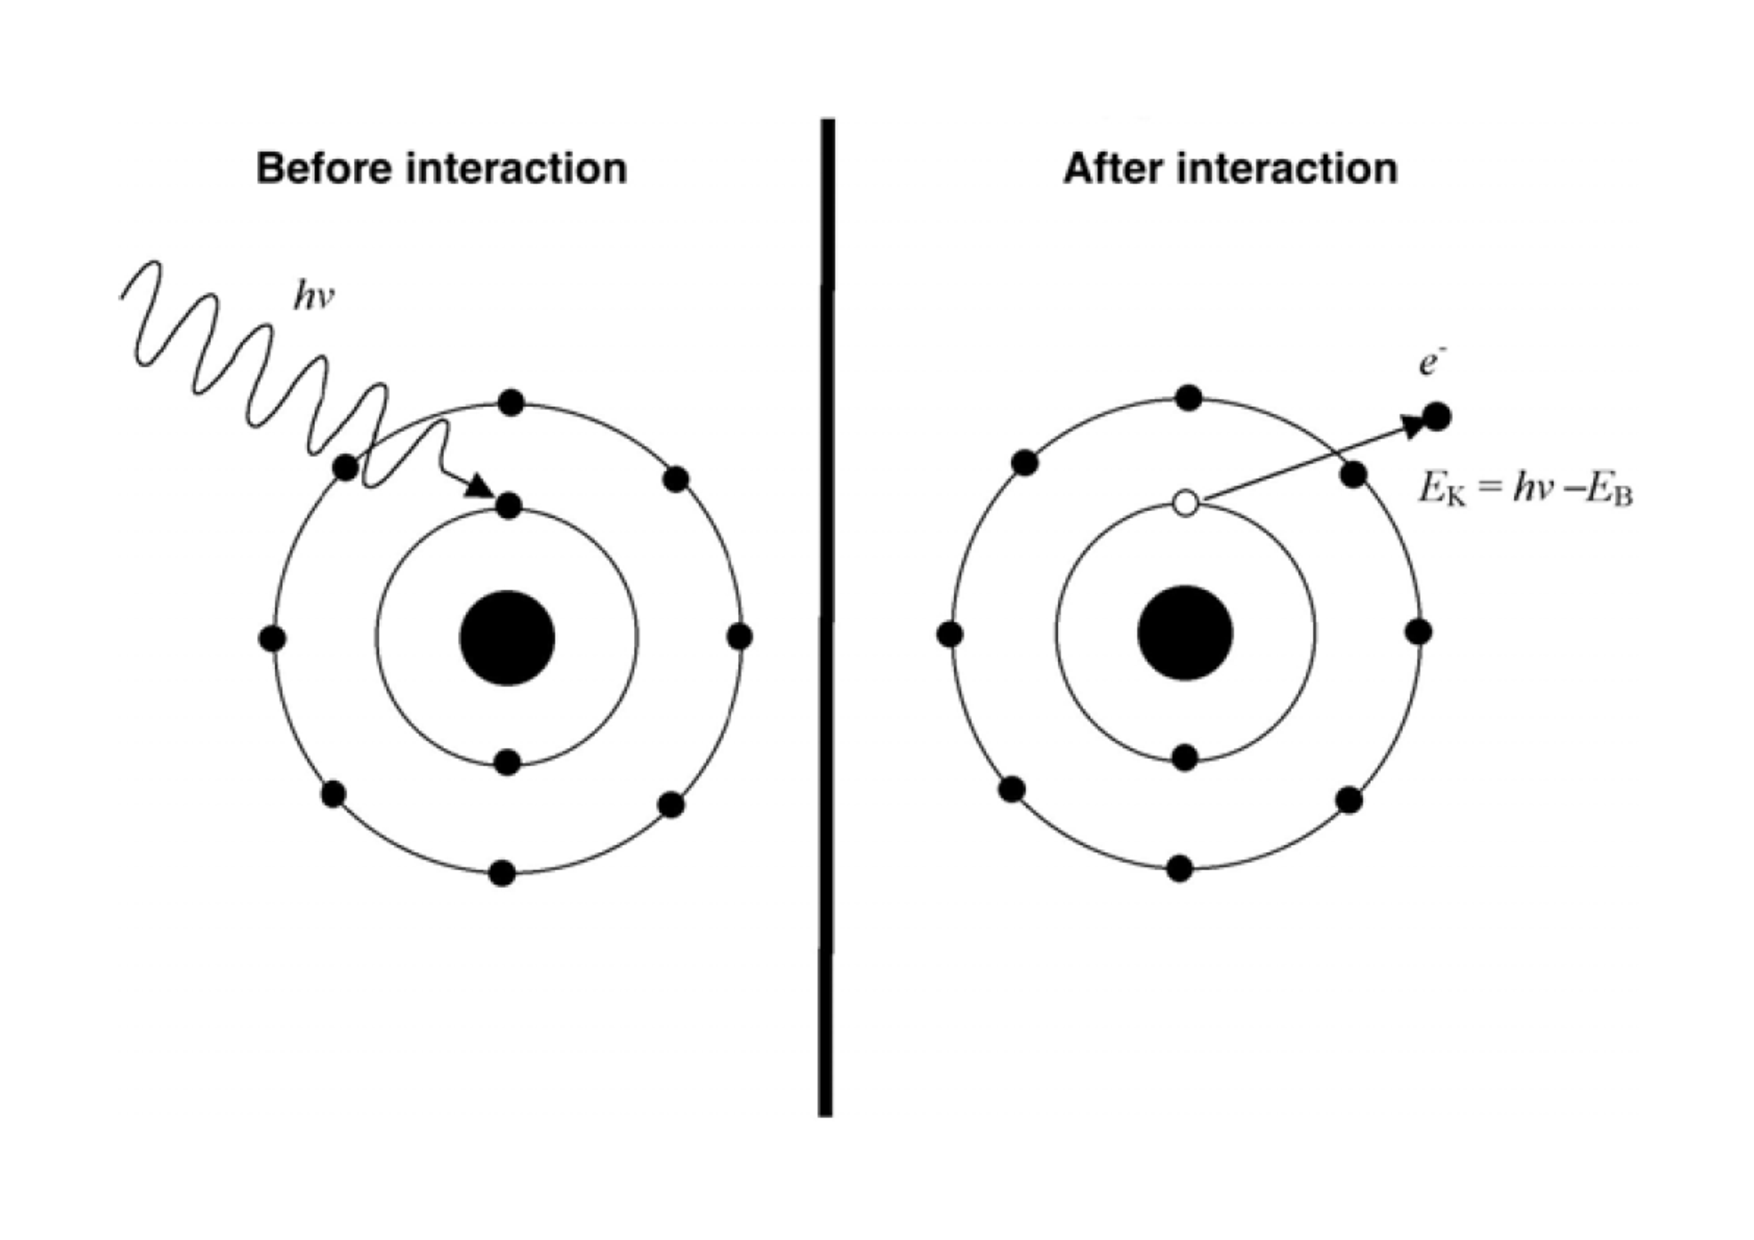
\includegraphics[width=0.8\textwidth]{03_GraphicFiles/chapter2_GammaCameras/photoelectric_abs.pdf}
\caption{Schematic diagram of the photoelectric effect. A photon with energy $h \nu$ interacts with a K-shell electron, which is ejected as photoelectron with kinetic energy $E_K$. In~\cite{Podgorsak2010}.}
\label{chap2::fig::photoel_abs}
\end{figure} 

The interaction is with the atom as a whole, and cannot take place with free electrons for conservation of energy and momentum constraints, although the whole photon energy is transferred to an atomic electron in one of the atom bound shells (tightly bound electron). Energy and momentum cannot be conserved simultaneously in a photon-free electron interaction: the momentum conservation requires a third object (the atom) involved in the interaction which must absorb the extra momentum. When the photon energy exceeds the K-shell binding energy of the absorber, about 80\% of all photoelectric absorption interactions occur with the K-shell electrons. If the energy transferred to the photoelectron is not below the binding energy threshold, it can be sufficient to raise it to a higher orbit, in a process of excitation. 
As a result of the photoelectric absorption, in addition to the ejected photoelectron, the absorber atom has a vacancy in one of its bound shells. This vacancy is quickly filled through capture of a free electron of the medium and/or rearrangement of electrons from other shells at higher energy level. Therefore, depending on the involved shells, one or more characteristics x-ray photons (fluorescent photons) may also be generated. Such photons are generally reabsorbed close to the original atom site through a further photoelectric absorption involving less tightly bound shells. In some fraction of the cases, the emission of an Auger electron may substitute for the characteristic x-ray in carrying away the atomic excitation energy. As the fluorescent photons, Auger electrons are generally reabsorbed very near the site of the original interaction.
The photoelectric process is the predominant mode of interaction for gamma rays of relatively low energy, and it is also enhanced for absorber materials of high atomic number Z. Even if a single analytic expression for the probability of photoelectric absorption over all ranges of photon energy $E_{\gamma}$ and Z, the probability ($\sigma_{PE}$)dependence on these two parameters can be approximated as shown in equation~\ref{chap2::eq::photoelProb}, where $n$ varies in the range [4,5] depending on the photon energy (4 for relatively low photon energies, 5 in the relativistic region)~\parencite{Knoll2000}.

\begin{equation}
\sigma_{PE} \varpropto \frac{Z^n}{E^{3.5}_{\gamma}} 
\label{chap2::eq::photoelProb}
\end{equation}  
 
In \figurename~\ref{chap2::fig::photonCrossSec} the cross section for the photoelectric absorption is compared to the one of the other photon interaction mechanisms for a copper absorber as a function of the photon energy. It exhibits a characteristic sawtooth structure in which the sharp discontinuities arise whenever the photon energy coincides with the binding energy of a particular electron shell. Except for the K shell, all other shells have a fine energy structure which reflect in the cross section curve.  

An interaction of a photon of energy $h\nu$ \myMarginnote{Compton scattering} with a loosely bound orbital electron of an absorber is called Compton scattering in honor of Arthur Compton who made the first measurements of photon-\enquote{free electron} scattering in 1923~\parencite{Compton1923}. Compton earned the Nobel prize for the discovery in 1927.  
In Compton scattering, the incoming gamma-ray photon is deflected through an angle $\theta$ with respect to its original direction, while transferring a portion of its energy to the electron, referred to as \enquote{recoil electron}. In theoretical studies of such an interaction mechanism, an assumption is made that the photon interacts with a free and stationary electron. As a result of the interaction, the photon, which had an initial energy $h\nu$, continue traveling in the new direction (angle $\theta$ with respect to the incident direction) with reduced energy $h\nu'$, and the recoil electron is ejected from the atom with a kinetic energy $E_K$ and a direction with an angle $\phi$ with respect the photon incident direction. A schematic view of the interaction is given in \figurename~\ref{chap2::fig::compton_principle}.
The expression that relates the energy transfer and the scattering angle for any given interaction can be derived by writing simultaneous equations for the conservation of energy and momentum. The obtained relationship is presented in equation~\ref{chap2::eq::Compton}, with the notation described above and $m_{0}c^2$ the rest-mass energy of the electron (511~keV). From the same calculation the kinetic energy of the recoil electron is also obtained from the expression in equation~\ref{chap2::eq::ComptonRecEnergy}.

\begin{equation}
h\nu' = \frac{h\nu}{1+\frac{h\nu}{m_{0}c^2}(1-\cos(\theta))}
\label{chap2::eq::Compton}
\end{equation} 

\begin{equation}
E_K = h\nu \frac{\frac{h\nu}{m_0c^2} (1-\cos(\theta))}{1+\frac{h\nu}{m_{0}c^2}(1-\cos(\theta))}
\label{chap2::eq::ComptonRecEnergy}
\end{equation} 

\begin{figure}[!htbp]
\centering
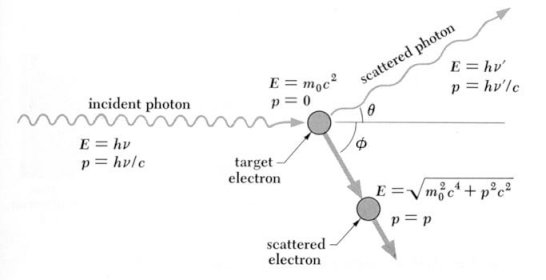
\includegraphics[width=0.8\textwidth]{03_GraphicFiles/chapter2_GammaCameras/ComptonPrinciple.jpg}
\caption{Schematic view of the Compton scattering principle. Image from https://universe-review.ca/R15-12-QFT10.htm.}
\label{chap2::fig::compton_principle}
\end{figure} 

From equation~\ref{chap2::eq::Compton} emerges how small scattering angles correspond to little energy transfers, and the other way around. In particular, for $\theta = 0$, no energy is transferred to the electron and the interaction becomes a classical Thomson scattering. For for $\theta > 0$ the energy of the scattered photon saturates at high values of the incident photon energy; the larger is the scattering angle, the lower is the saturation value of $h\nu'$ for $h\nu \lim \infty$
The relationship between the photon energy before and after the interaction is shown in \figurename~\ref{chap2::fig::ComptonEnergy} for various scattering angles $\theta$ between 0\textdegree (forward scattering) and $\pi$ (back-scattering.) 
The scattering angle $\theta$ and the recoil electron angle $\phi$ are related by equation~\ref{chap2::eq::ComptonAngles}.

\begin{equation}
\cot(\phi) = (1+\frac{h\nu}{m_{0}c^2})\tan\bigg(\frac{\theta}{2}\bigg)
\label{chap2::eq::ComptonAngles}
\end{equation} 

This relationship shows that for a given $\theta$, the higher is the incident photon energy $h\nu$, the smaller is the recoil electron angle $\phi$. In \figurename~\ref{chap2::fig::thetaphirel} the scattering and recoil angle dependence is plotted for different values of $\epsilon = h\nu / m_{0}c^2$.

\begin{figure}
\centering
\begin{subfigure}[t]{.49\textwidth}
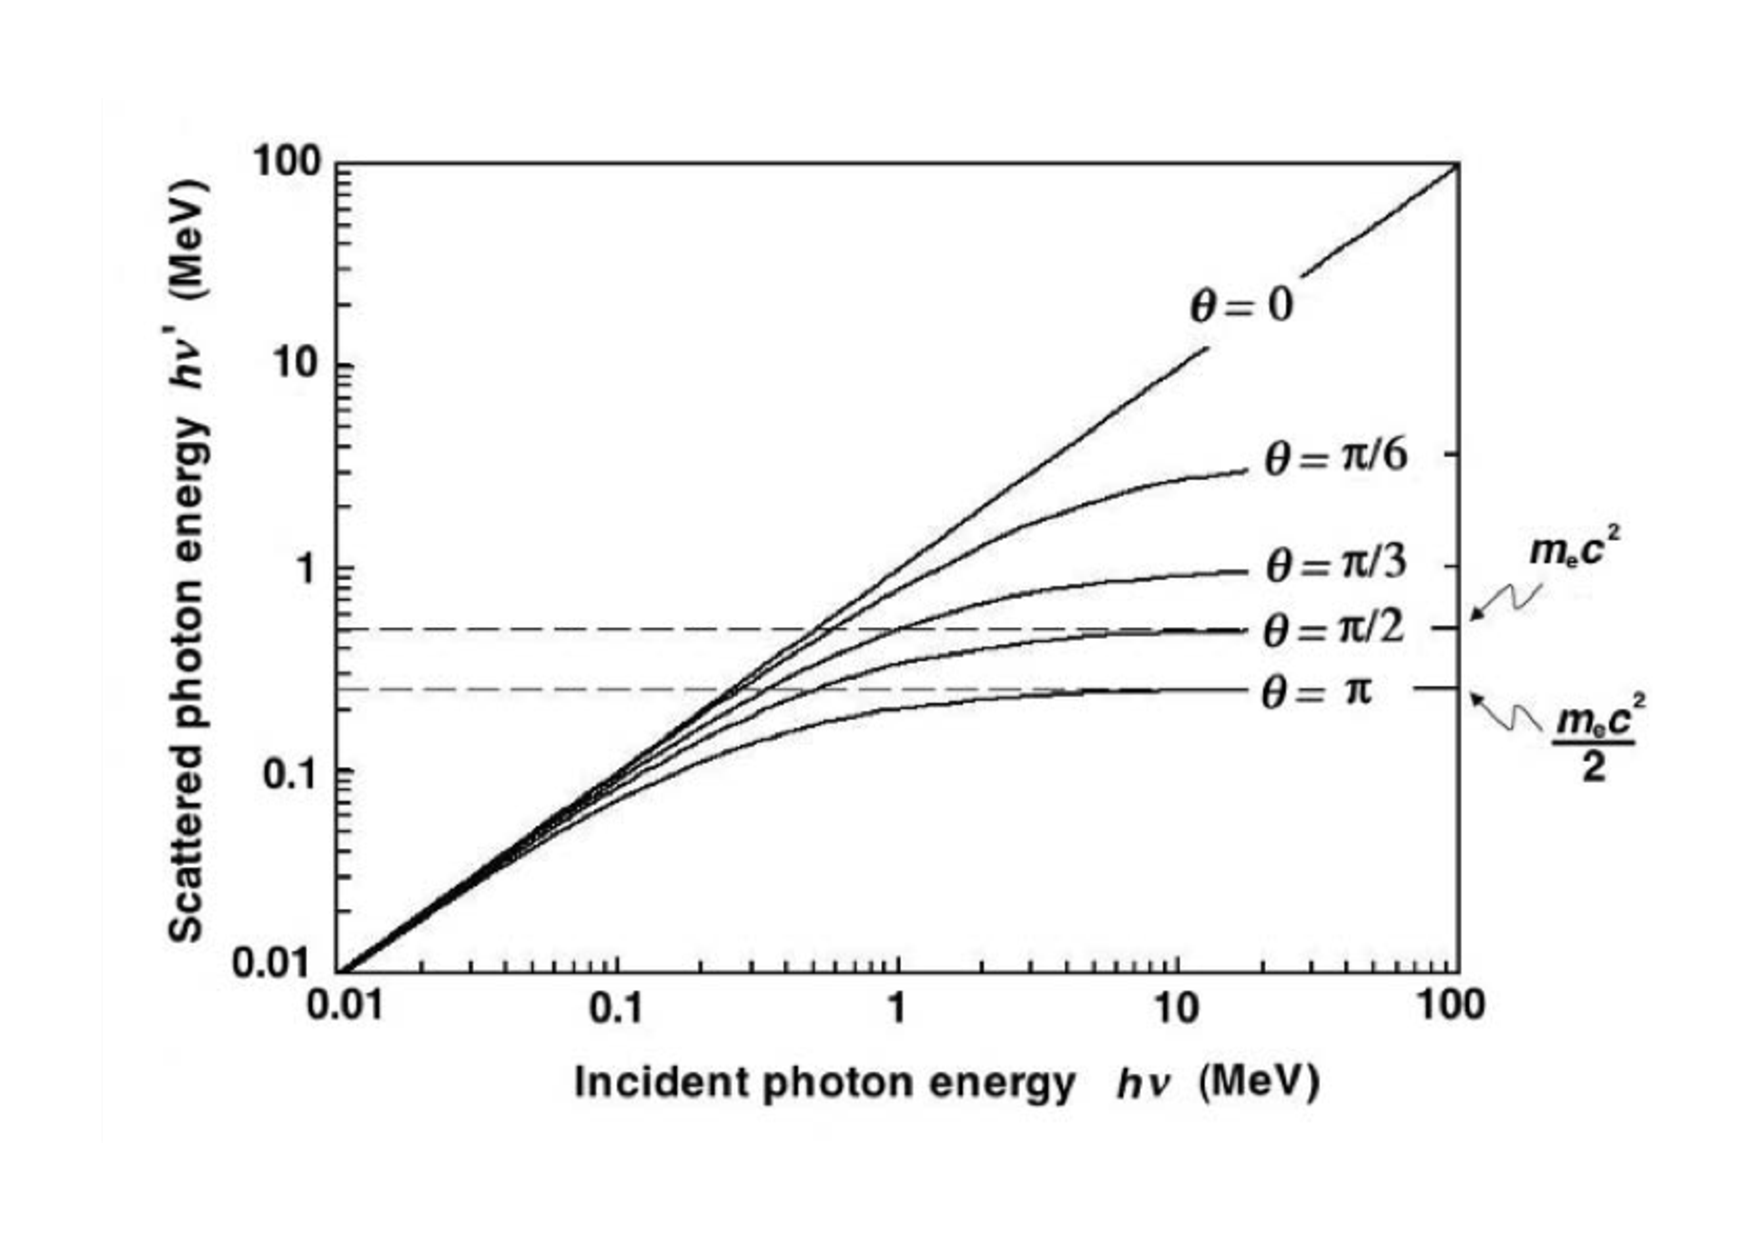
\includegraphics[width=1.1\linewidth]{03_GraphicFiles/chapter2_GammaCameras/ComptonEnergy.pdf}
\caption{Scattered photon energy against the incident photon energy for various Compton scattering angles in the range from 0\textdegree to $\pi$.}
\label{chap2::fig::ComptonEnergy}
\end{subfigure}
\begin{subfigure}[t]{.49\textwidth}
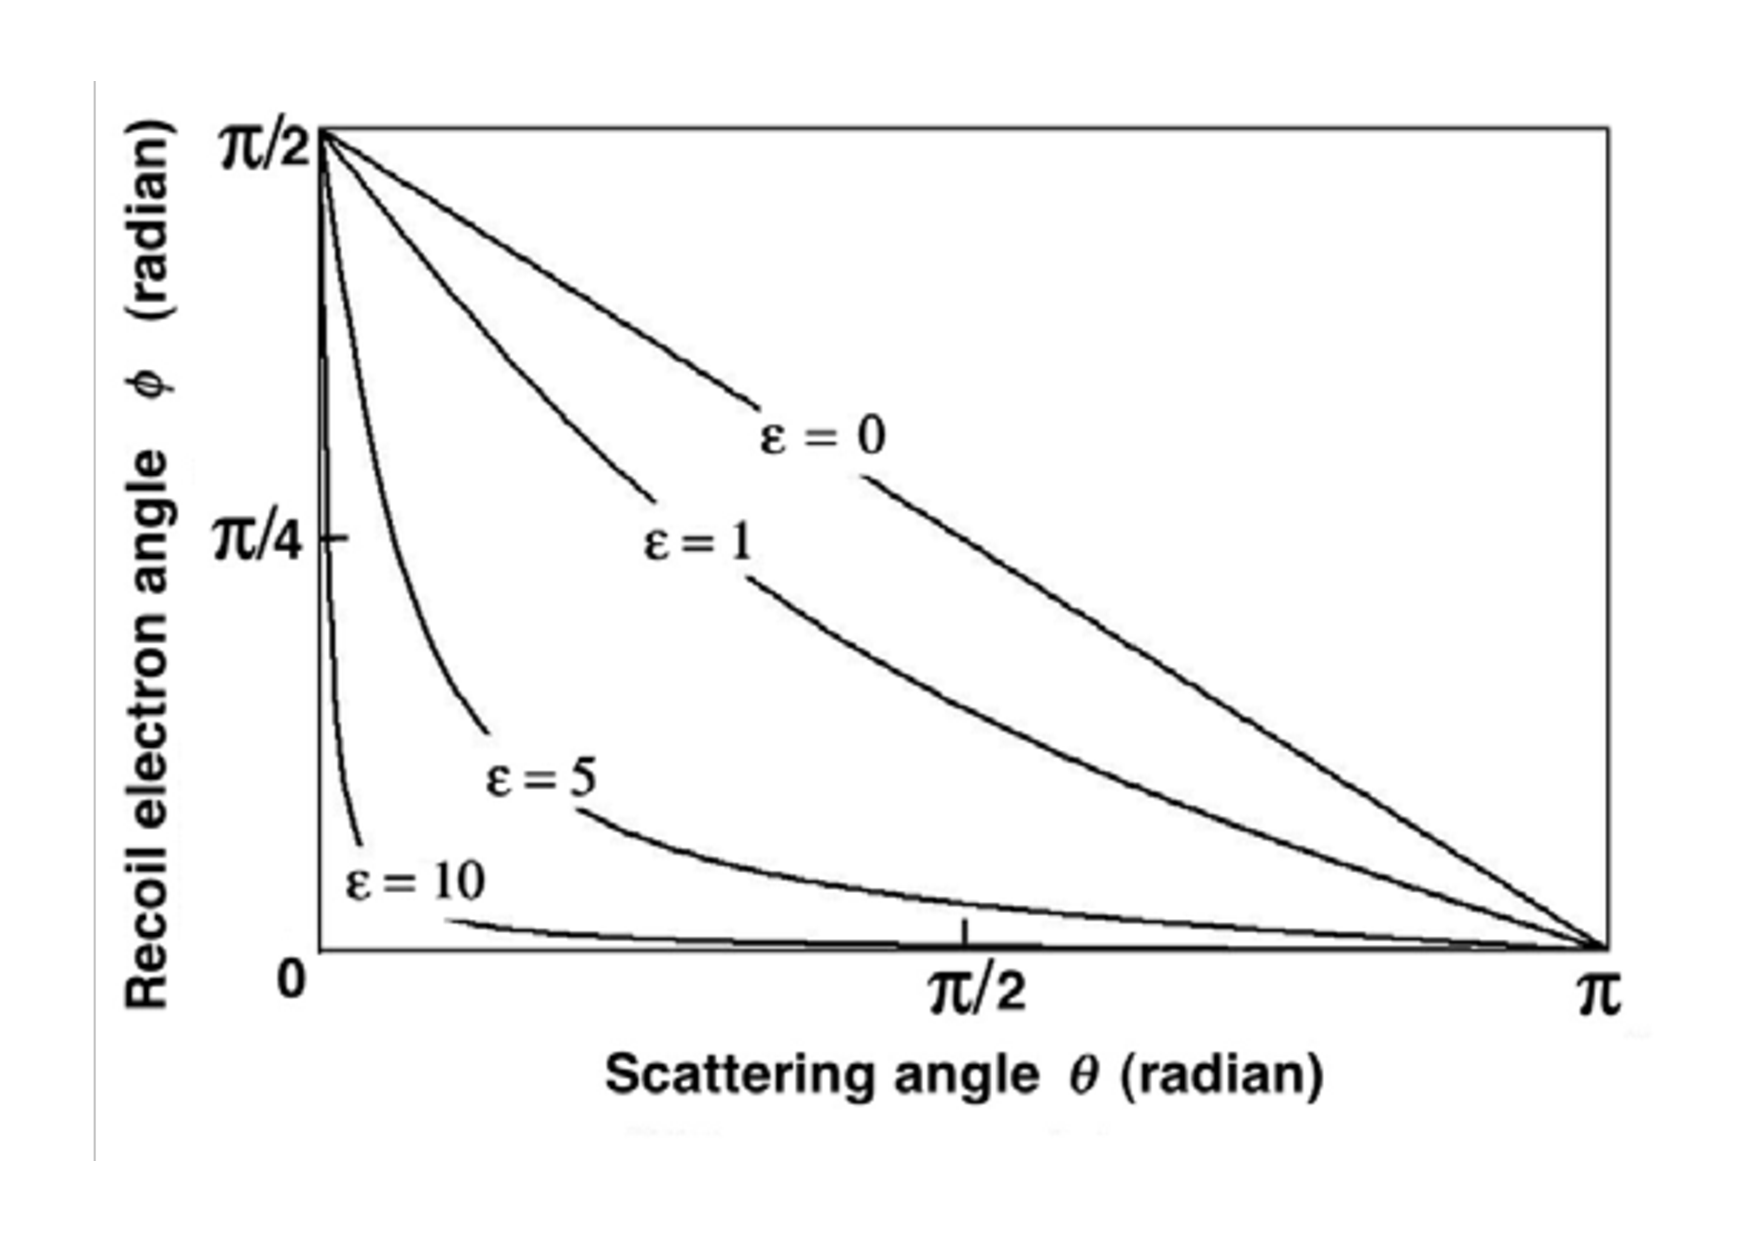
\includegraphics[width=1.1\linewidth]{03_GraphicFiles/chapter2_GammaCameras/scattRecoilAnglesCompton.pdf}
\caption{Relationship between the electron recoil electron $\phi$ and the photon Compton scattering angle $\theta$.}
\label{chap2::fig::thetaphirel}
\end{subfigure}
\caption{In~\cite{Podgorsak2010}}
\label{chap2::fig::ComptonAngular}
\end{figure}
   
The probability of Compton scattering per atom of the absorber depends on the number of electrons available as scattering targets and therefore linearly increases with the atomic number Z. In \figurename~\ref{chap2::fig::photonCrossSec} the probability energy dependence is shown for a copper target and compared to the other interaction channels probability. The differential cross section, or angular distribution of scattered gamma rays, is predicted by a formula derived by Oskar Klein and Yoshio Nishina in 1929, and reported in equation~\ref{chap2::eq::KleinNishina}~\parencite{Klein1929}.
 \begin{equation}
\frac{\mathrm{d}\sigma}{\mathrm{d}\Omega} = Zr_{e}\bigg(\frac{1}{1+\epsilon (1-\cos(\theta))}\bigg)^{2}\bigg( \frac{1+\cos^2(\theta)}{2} \bigg)\bigg(1+\frac{\epsilon^2(1-\cos(\theta))^2}{(1+\cos^2(\theta)[1+\epsilon(1-\cos(\theta))])} \bigg) 
\label{chap2::eq::KleinNishina}
\end{equation} 
where $r_{e}$ is the classical electron radius expressed in equation~\ref{chap1::eq::electronRad}. The distribution is shown graphically in \figurename~\ref{chap2::fig::ComptonAngCrossSection} and illustrates the strong tendency for forward scattering at high values of the gamma-ray energy. At low incident photon energies the probability for forward scattering and back-scattering are equal and twice as large as the probability for side scattering. As the incident photon energy increases, the scattering becomes increasingly more forward peaked and back-scattering rapidly diminishes.

\begin{figure}[!htbp]
\centering
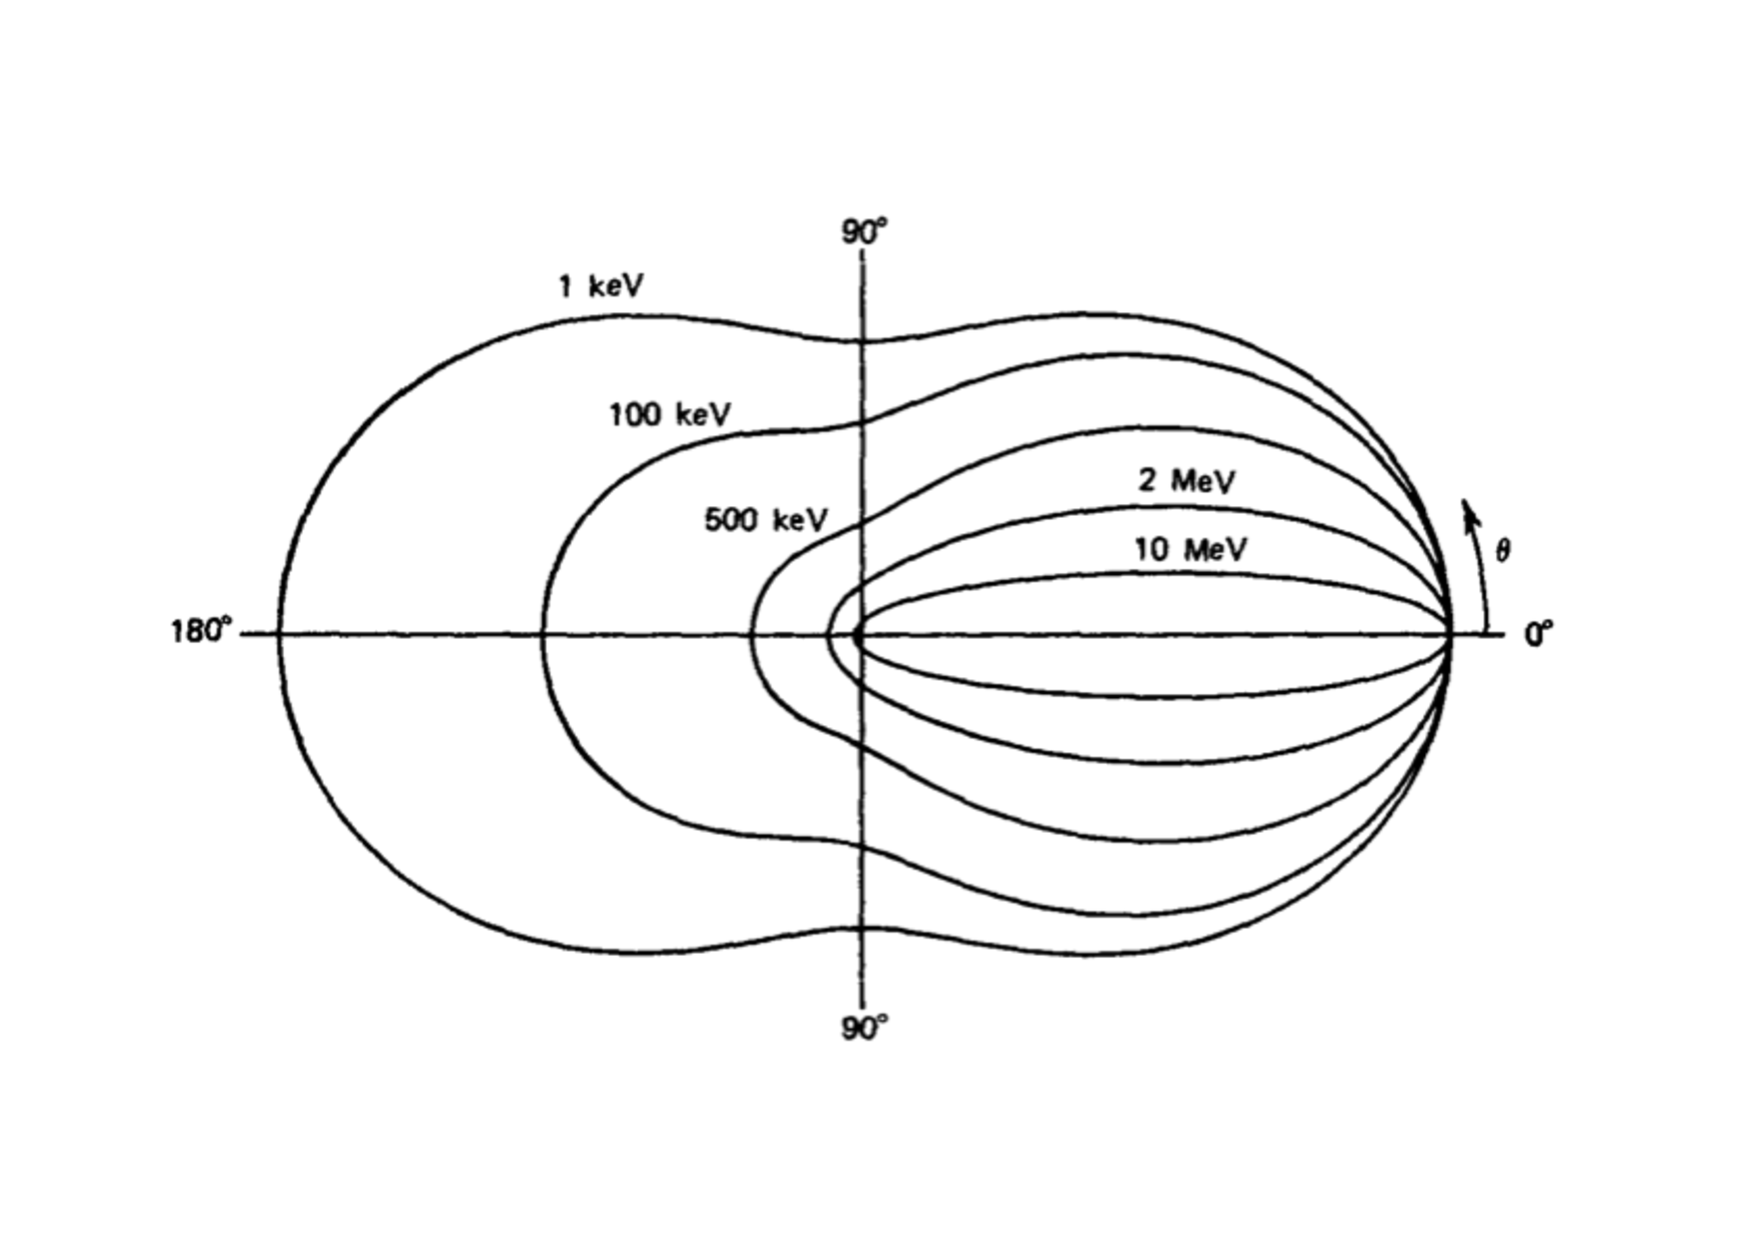
\includegraphics[width=0.8\textwidth]{03_GraphicFiles/chapter2_GammaCameras/ComptonPolar.pdf}
\caption{Polar plot of the number of photons (incident from the left side) Compton scattered into a unit solid angle at the scattering angle $\theta$, for the different indicated incident photon energies. In~\cite{Knoll2000}.}
\label{chap2::fig::ComptonAngCrossSection}
\end{figure}
 
As mentioned, the Compton cross section and energy transfer are calculated with the assumption of free electrons, but at very low incident photon energies such an assumption breaks down and the electronic binding energy $E_B$ affects the Compton interaction: the closer is the photon energy $h\nu$ to $E_B$, the larger is the deviation of the atomic cross section from the one calculated with the Klein-Nishina formula. Various theories have been developed to account for electronic binding energy effects and apply corrections on the Compton atomic cross sections~\parencite{Bergstrom1997}. It is worth to notice that for a given absorber Z, the binding energy correction is more significant at lower photon energies, and for a given initial energy $h\nu$, the binding energy correction is more significant at higher atomic number Z. The described binding energy effect is also referred to as \enquote{Doppler broadening}~\parencite{DuMond1928, DuMond1929}. 
   
If the photon incident energy exceeds twice the the rest-mass energy of and electron \myMarginnote{Pair production} $2m_ec^2 = $ 1.02~MeV, the production of an electron-positron pair in conjunction with a complete absorption of the photon becomes energetically possible. In practice, as shown in \figurename~\ref{chap2::fig::photonCrossSec},  the probability of such an interaction mechanism, referred to as pair production, remains very low until the gamma-ray energy approaches several MeV and therefore pair production is predominantly confined to high-energy photons. For $h\nu > 2m_ec^2$, energy and charge can be conserved even if pair production occurs in free space, but the conservation of linear momentum requires the Coulomb field of a collision partner (atomic nucleus or orbital electron). The photon, indeed, possesses momentum excess that is not absorbed by the electron-positron pair, and must be absorbed by the collision partner. When such an extra momentum is absorbed by the atomic nucleus, the recoil energy, as a result of the relatively large nuclear mass, is exceedingly small and the effect is described as the standard pair production: the incident gamma-ray disappears and is replaced by an electron-positron pair. When an orbital electron of the atom picks up the extra momentum, the recoil energy may be significant and determine the ejection of the orbital electron; in this case, the photon is absorbed and three particles leaves the interaction site, two electrons and a positron, in the so-called \enquote{triplet production}. A schematic representation of these two effects is given in \figurename~\ref{chap2::fig::pairprod}.

\begin{figure}[!htbp]
\centering
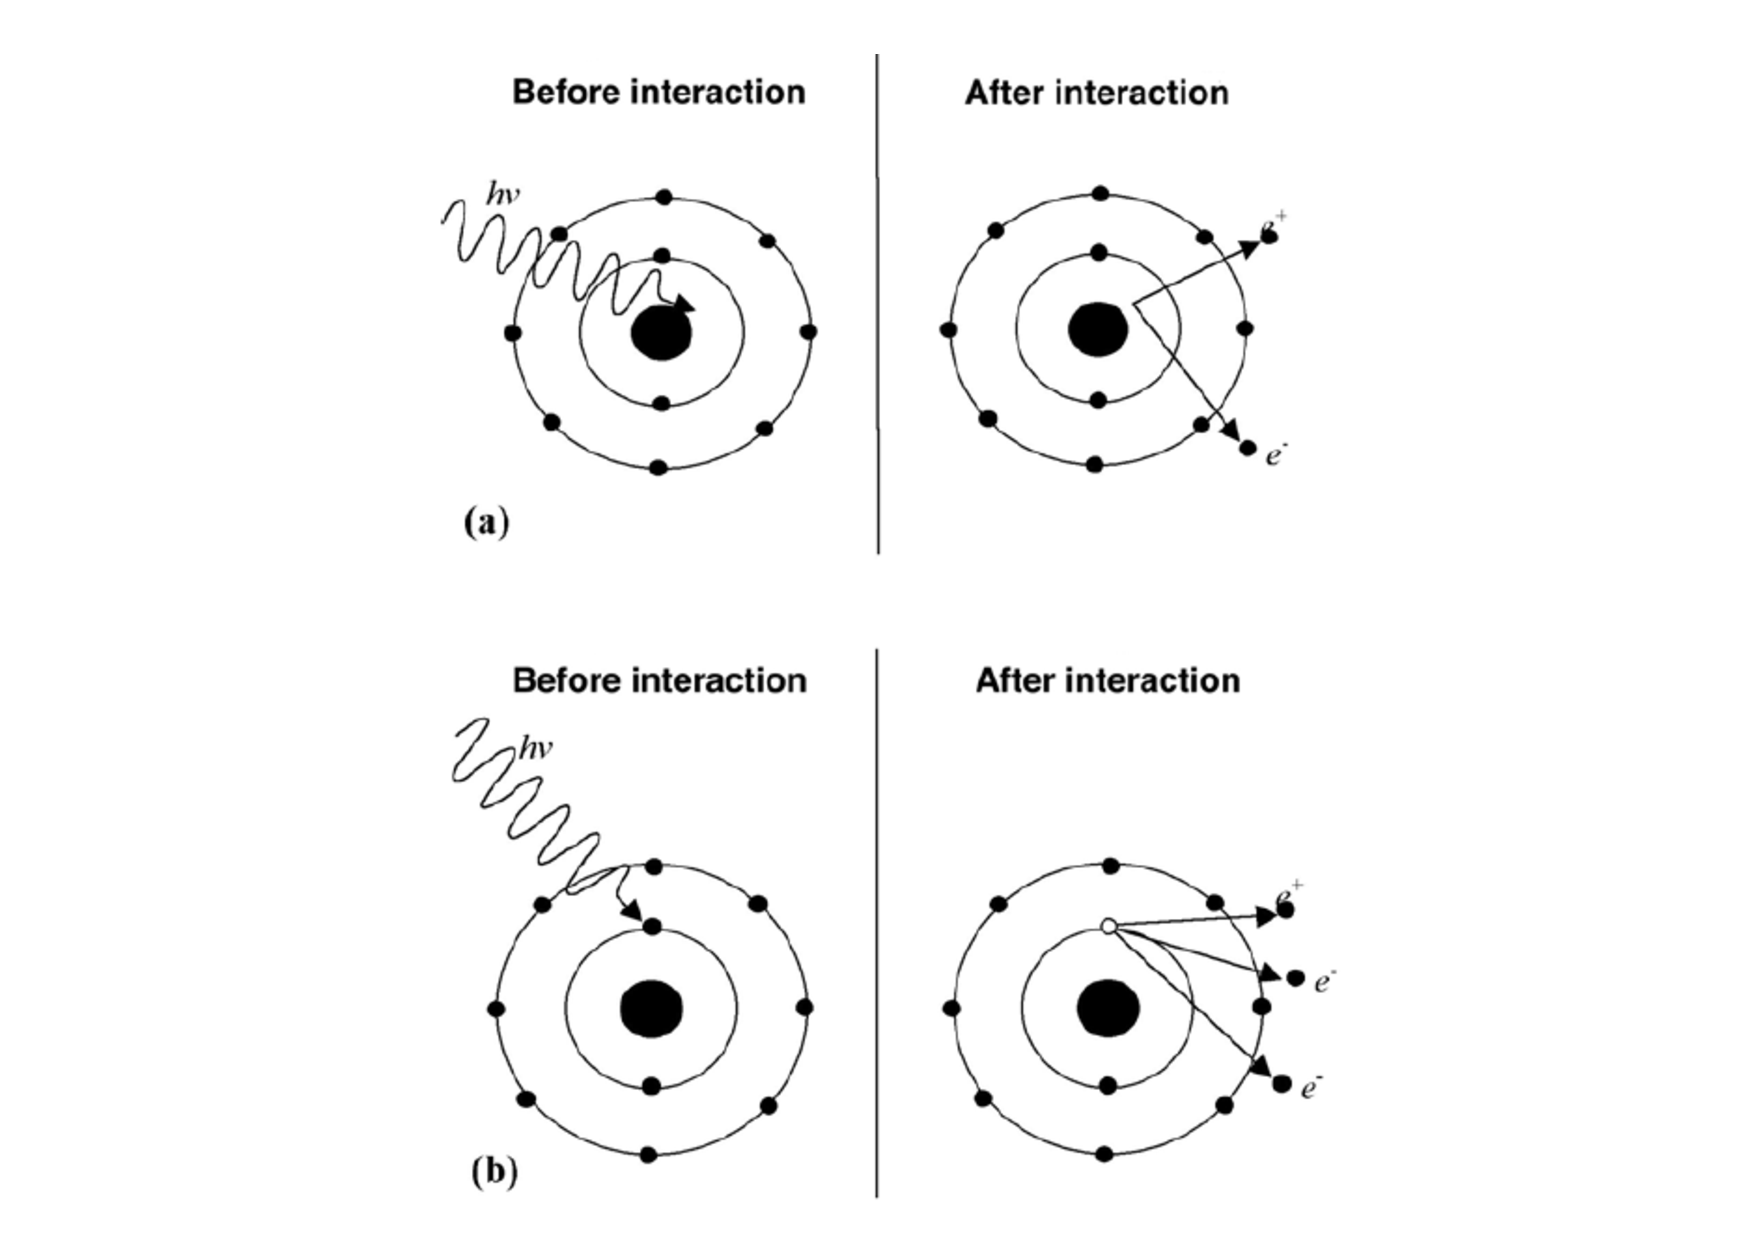
\includegraphics[width=0.9\textwidth]{03_GraphicFiles/chapter2_GammaCameras/pairProd.pdf}
\caption{Schematic representation of pari production (a) in the COulomb field of a nucleus and triplet production (b) in the Coulomb field of an orbital electron. In~\cite{Podgirsak2010}.}
\label{chap2::fig::pairprod}
\end{figure} 

The total kinetic energy transferred to the charged particles is the difference between the photon incident energy and twice the rest-mass energy of the positron-electron pair.
In both cases, because the positron will annihilate after slowing down in the absorbing medium, two annihilation photons are normally produced as secondary products of the interaction. 
No simple expression exists for the probability of pair production per nucleus, but its magnitude varies approximately as the square of the absorber atomic number Z, and it rises sharply with the photon energy. 

\begin{figure}[!htbp]
\centering
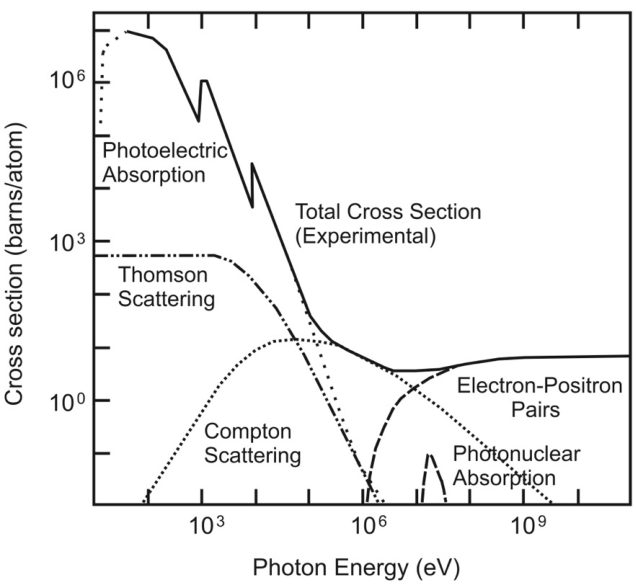
\includegraphics[width=0.8\textwidth]{03_GraphicFiles/chapter2_GammaCameras/Photon-energy-dependent-cross-sections-Cross-sections-of-the-photoelectric-absorption.png}
\caption{Cross sections of the photoelectric absorption, Thomson scattering, Compton scattering, pair production (electron-positron pairs), and photonuclear absorption for a copper absorber as a function
of the photon energy energy. In~\cite{Hermanss2013}.}
\label{chap2::fig::photonCrossSec}
\end{figure} 

The relative importance of the three described interaction processes for different absorber materials (Z) and gamma-ray energies ($h\nu$) are illustrated in \figurename~\ref{chap2::fig::relativePhotonInt}. Three areas are defined by the two solid lines in the plot, which indicates the energy/Z values for which the two neighboring effects have equivalent probability. 
 
\begin{figure}[!htbp]
\centering
\includegraphics[width=0.8\textwidth]{03_GraphicFiles/chapter2_GammaCameras/RelativePhotonInt.pdf}
\caption{Relative importance of the three major types of photon interaction in matter. The lines show the values of Z and $h\nu$ for which the two neighboring effects are just equal. In~\cite{Knoll2000}.}
\label{chap2::fig::relativePhotonInt}
\end{figure} 


If we now consider a photon beam interacting with a target, all the mentioned interaction processes removes gamma-ray photons from the beam either by absorption or by scattering away from the beam direction, and can be characterized by a fixed probability of occurrence per unit path length in the absorber. The sum of these probabilities is simply the probability per unit path length that the photon is lost and is referred to as \enquote{linear attenuation coefficient} $\mu$. Ther number of transmitted photons $I$ can be then expresses in terms of the number of incident photons in the beam $I_0$ as a function of the linear attenuation coefficient and the absorber thickness $t$, as shown by equation~\ref{chap2::eq::attenuation}.

 \begin{equation}
\frac{I}{I_0} = e^{-\mu t}
\label{chap2::eq::attenuation}
\end{equation} 

The average distance traveled by the a photon of the beam in the absorber before an interaction takes place is called \enquote{mean free path} $\lambda$, and is the reciprocal of the linear attenuation coefficient. In solids, for common gamma-ray energies, $\lambda$ can vary in the range between few millimeters to tens of centimeters. 
A more widely used parameter is the \enquote{mass attenuation coefficient} $\mu_{\rho}$, which normalize the linear attenuation coefficient to the absorber density $\rho$ (equation~\ref{chap2::eq::massAttenuation}).

\begin{equation}
\mu_{\rho} = \frac{\mu}{\rho}
\label{chap2::eq::massAttenuation}
\end{equation} 

If the mass attenuation coefficient is used, the convenient concept of mass thickness is also introduced, corresponding to the product of the absorber thickness $t$ by its density $\rho$ and generally measured in mg/cm$^2$. For compound and mixtures, the mass attenuation coefficient is approximated by a summation of a weighted average of its constituent, as expressed in equation~\ref{chap2::eq::massAttCoeffCompoud}.

 \begin{equation}
\mu_{\rho} = \sum_i{w_i\frac{\mu_i}{\rho}}
\label{chap2::eq::massAttCoeffCompoud}
\end{equation} 

with $w_i$ the proportion by weight of the i-th constituent, and $\mu_i/rho$ its mass attenuation coefficient. The attenuation coefficients have specific values for a given photon energy $h\nu$ and absorber atomic number Z, and are tabulated on the \gls{nist} database according to the calculations in~\cite{Seltzer1993}.

\section{Ion range monitoring with prompt-gamma radiation}\label{chap2::sec::PGionRangeMonitoring}

As introduced in chapter~\ref{chap::1}, the high ballistic precision of particle therapy is advantageous because it provides high dose selectivity while sparing the healthy tissues surrounding the tumors, but at the same time it makes such a cancer care modality quite sensitive to any source of uncertainty and deviation with respect to the treatment planning: patient mispositioning, organ motion or anatomical between fractions (such as tumor shrinking, weight loss, cavity filling). A reduction of the safety margins presently applied to the \gls{ptv} to account for such uncertainties would be only possible with the availability of a real-time range monitoring system. As the primary beam stops inside the patient, the range control should be based on secondary radiations issued from nuclear reactions. In particular, the work presented in this thesis is focused on range monitoring techniques relying on the detection of \gls{pg} rays.
 
\subsection{Prompt-gamma emission during particle therapy}\label{chap2::subsec::PGproduction}

The \gls{pg} range monitoring techniques rely on the emission of photons due to the relaxation of excited nuclei within about one nanosecond after the nuclear interaction. The \glspl{pg} are emitted in the whole solid angle around the patient and in a wide energy range (from some hundreds of keV up to 10 MeV). Such a prompt radiation has been demonstrated to be correlated to the ion range for both protons and carbon ions. It can be exploited via single photon detection systems to provide a real-time feedback in case of major deviations of the measured range with respect to the planned one, and eventually trigger a treatment emergency stop.

\begin{figure}
\centering
\begin{subfigure}[t]{.49\textwidth}
\hspace{-1cm}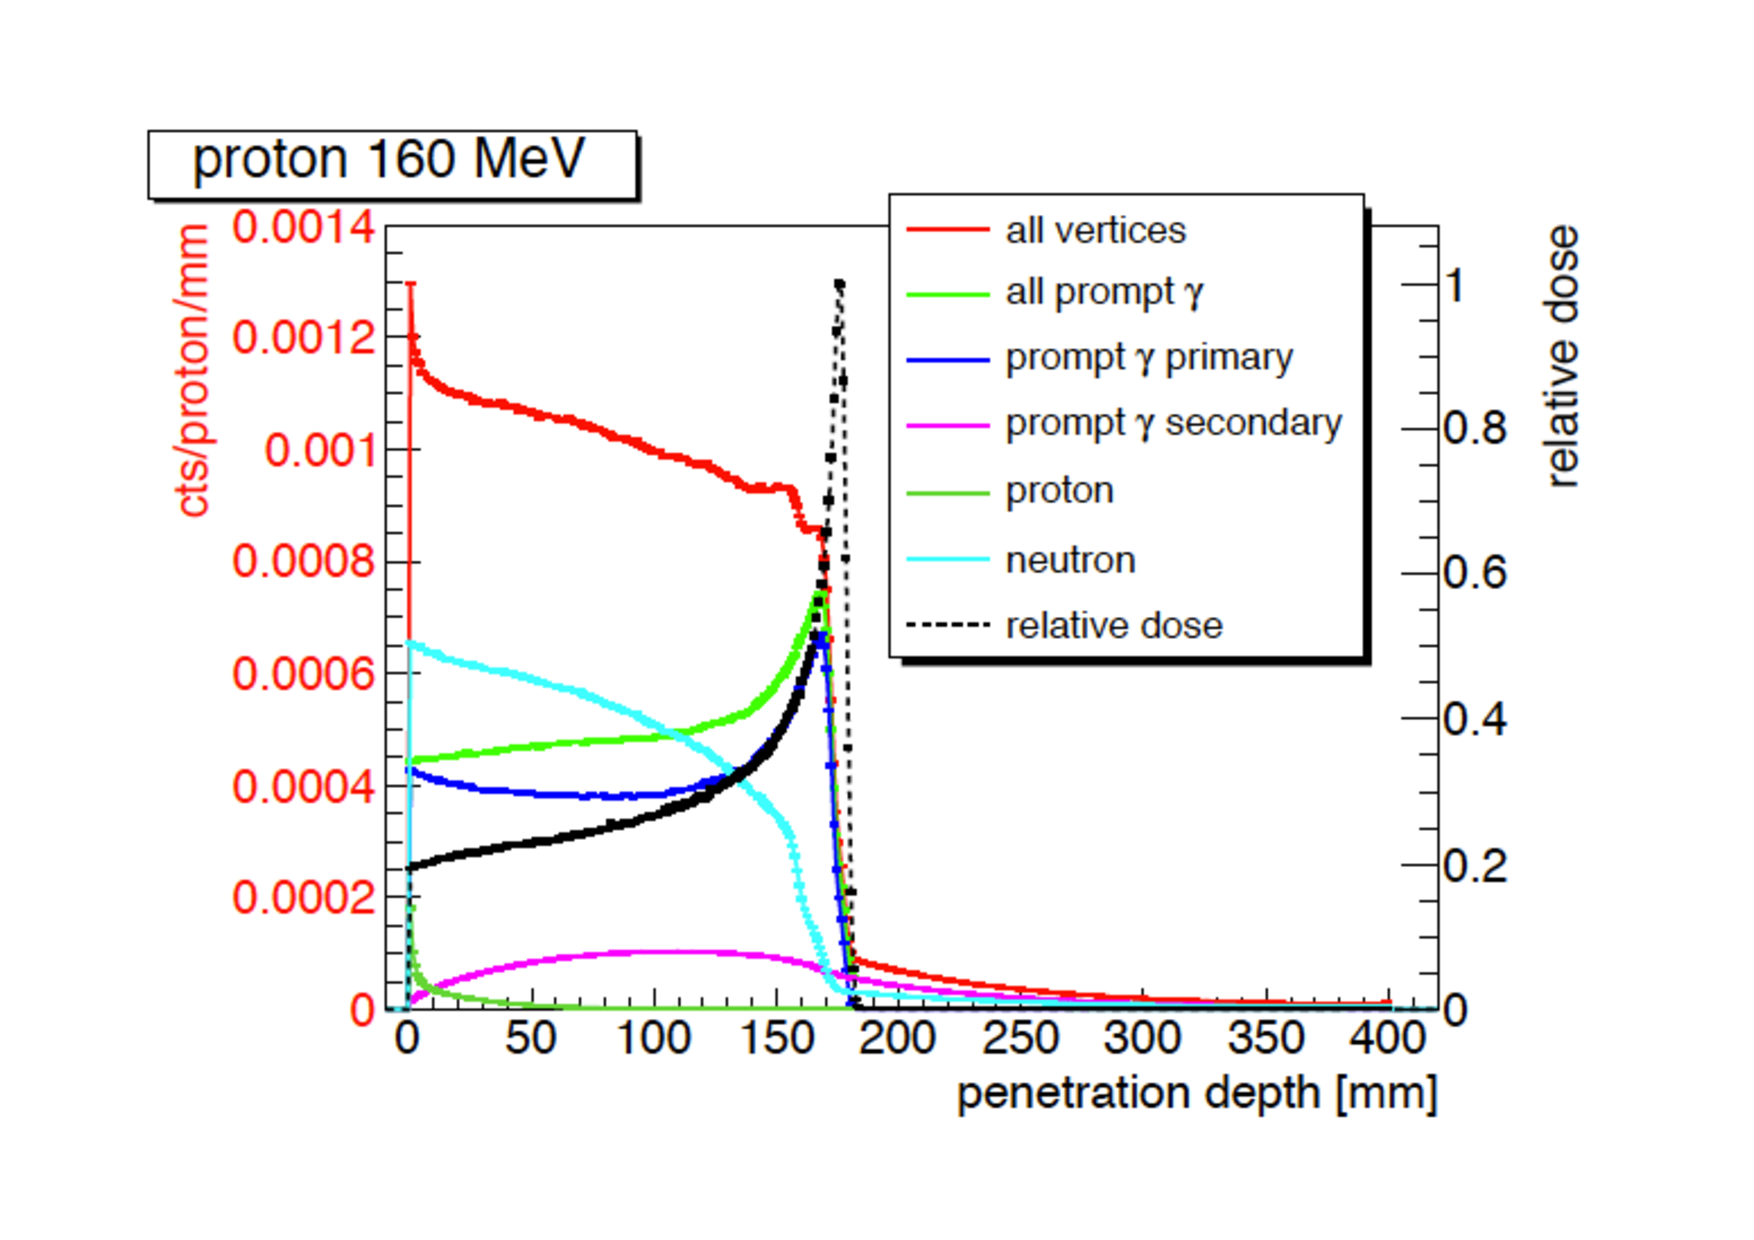
\includegraphics[width=1.3\linewidth]{03_GraphicFiles/chapter2_GammaCameras/PG_secPartDistr_p.pdf}
\caption{Emission vertices of secondary particles emerging from a cylindrical water target (15~cm diameter, 40~cm length) irradiated by a 160~MeV proton beam. An energy lower threshold of 1~MeV has been applied.}
\label{chap2::fig::PGsecDistrp}
\end{subfigure}
\begin{subfigure}[t]{.49\textwidth}
\hspace{-1cm}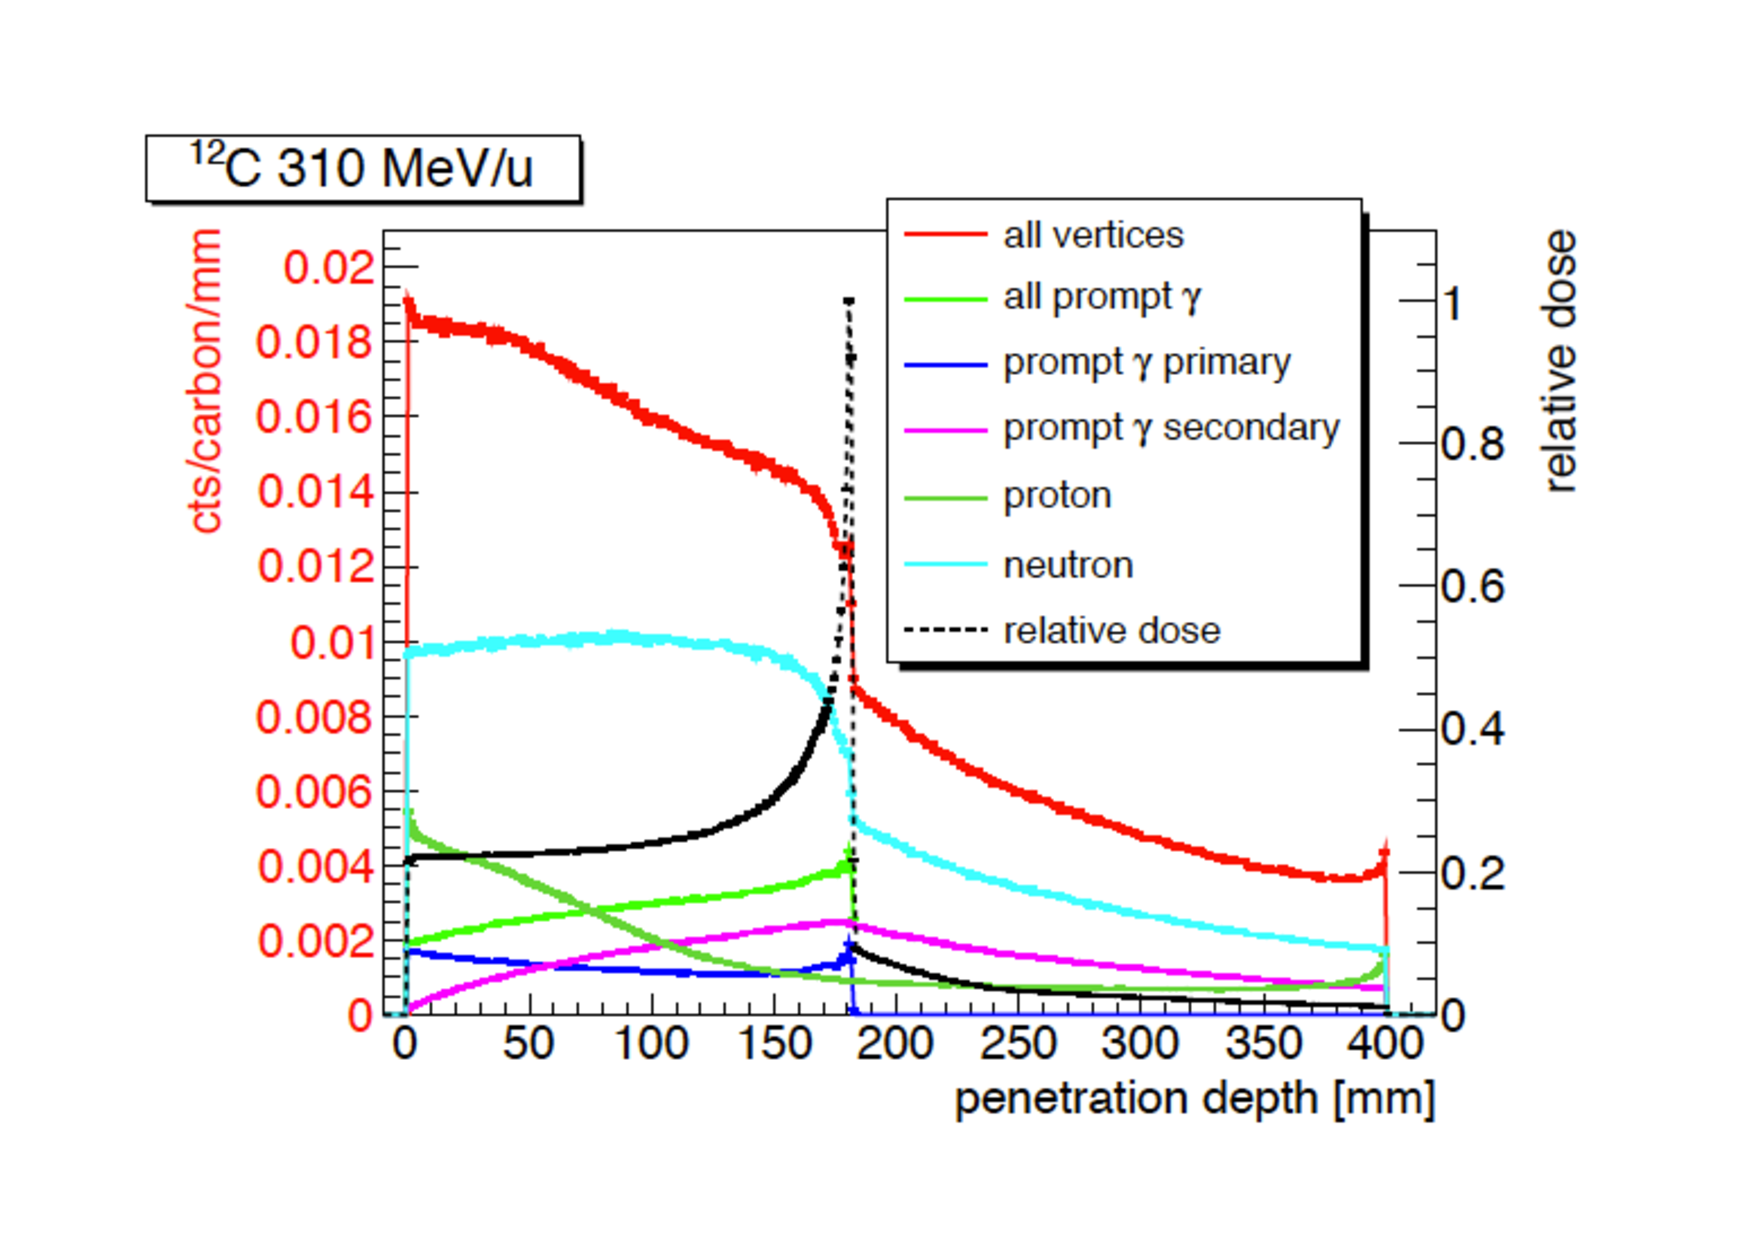
\includegraphics[width=1.3\linewidth]{03_GraphicFiles/chapter2_GammaCameras/PG_secPartDistr_C.pdf}
\caption{Emission vertices of secondary particles emerging from a cylindrical water target (15~cm diameter, 40~cm length) irradiated by a 310~MeV/u carbon ion beam. An energy lower threshold of 1~MeV has been applied.}
\label{chap2::fig::PGsecDistrC}
\end{subfigure}
\caption{In~\cite{Krimmer2017}.}
\label{chap2::fig::PGsecDistr_gen}
\end{figure}

\figurename~\ref{chap2::fig::PGsecDistr_gen} shows the distribution of emission vertices \myMarginnote{PG spatial features} of secondary radiation emitted by an homogeneous water phantom (cylinder of 15~cm diameter and 40~cm length) in the beam direction, together with the dose profile. The simulated data have been obtained by irradiating the phantom with 160~MeV protons (\figurename~\ref{chap2::fig::PGsecDistrp}) and 310~MeV/u carbon ions (\figurename~\ref{chap2::fig::PGsecDistrp}), having the same expected range in water. All the secondary particle vertex distributions are correlated to the primary ion range, and in particular \glspl{pg} appear as the best candidates for range monitoring purpose, given the significant emitted statistics. Also neutrons are produced in considerable fraction, mainly in carbon ion irradiation, but the spatial information about their production vertex is hardly retrievable.  The correlation between longitudinal \gls{pg} and dose profiles can be exploited for \enquote{imaging} monitoring approaches lo locate the Bragg peak position. Physically and electronically collimated prototypes are used to access the spatial information carried by the emitted photons, and will be described in following sections. 
In addition to the spatial information, also energy and timing \gls{pg} specific features can be used as tools to retrieve the Bragg peak position with the so-called \enquote{non-imaging techniques}. The wide energy spectrum of the produced \gls{pg} rays \myMarginnote{PG energy distribution} depends on the composition of the target material, and it is characterized by discrete lines. In \figurename{chap2::fig::PGEdistr}, the \gls{pg} energy spectrum is shown for the simulated irradiation of \gls{pe}, \gls{pmma} and water targets with a 160~MeV proton beam. The discrete spectroscopic lines are clearly visible: in particular, three lines are highlighted, corresponding to the de-excitation of $^{16}$O (6.13~MeV), $^{12}$C (4.44~MeV), and deuterium (2.22~MeV). The latter is the result of neutron capture by hydrogen, and the produced photon distribution is not correlated to the primary particle range. The comparison of the measured \gls{pg} energy spectrum to the expected one can be used to access information about the material traversed by the primary beam and estimate the proton range: such a technique is referred to as \gls{pgs}~\parencite{Verburg2014}, and will be further discussed in following sections. To be noticed that the \gls{pg} yields are not only depending on the traversed material composition, but also on the beam energy; a global enhancement is observed as the energy decreases~\parencite{Krimmer2017}.  

\begin{figure}
\centering
\begin{subfigure}[t]{.49\textwidth}
\hspace{-1.cm}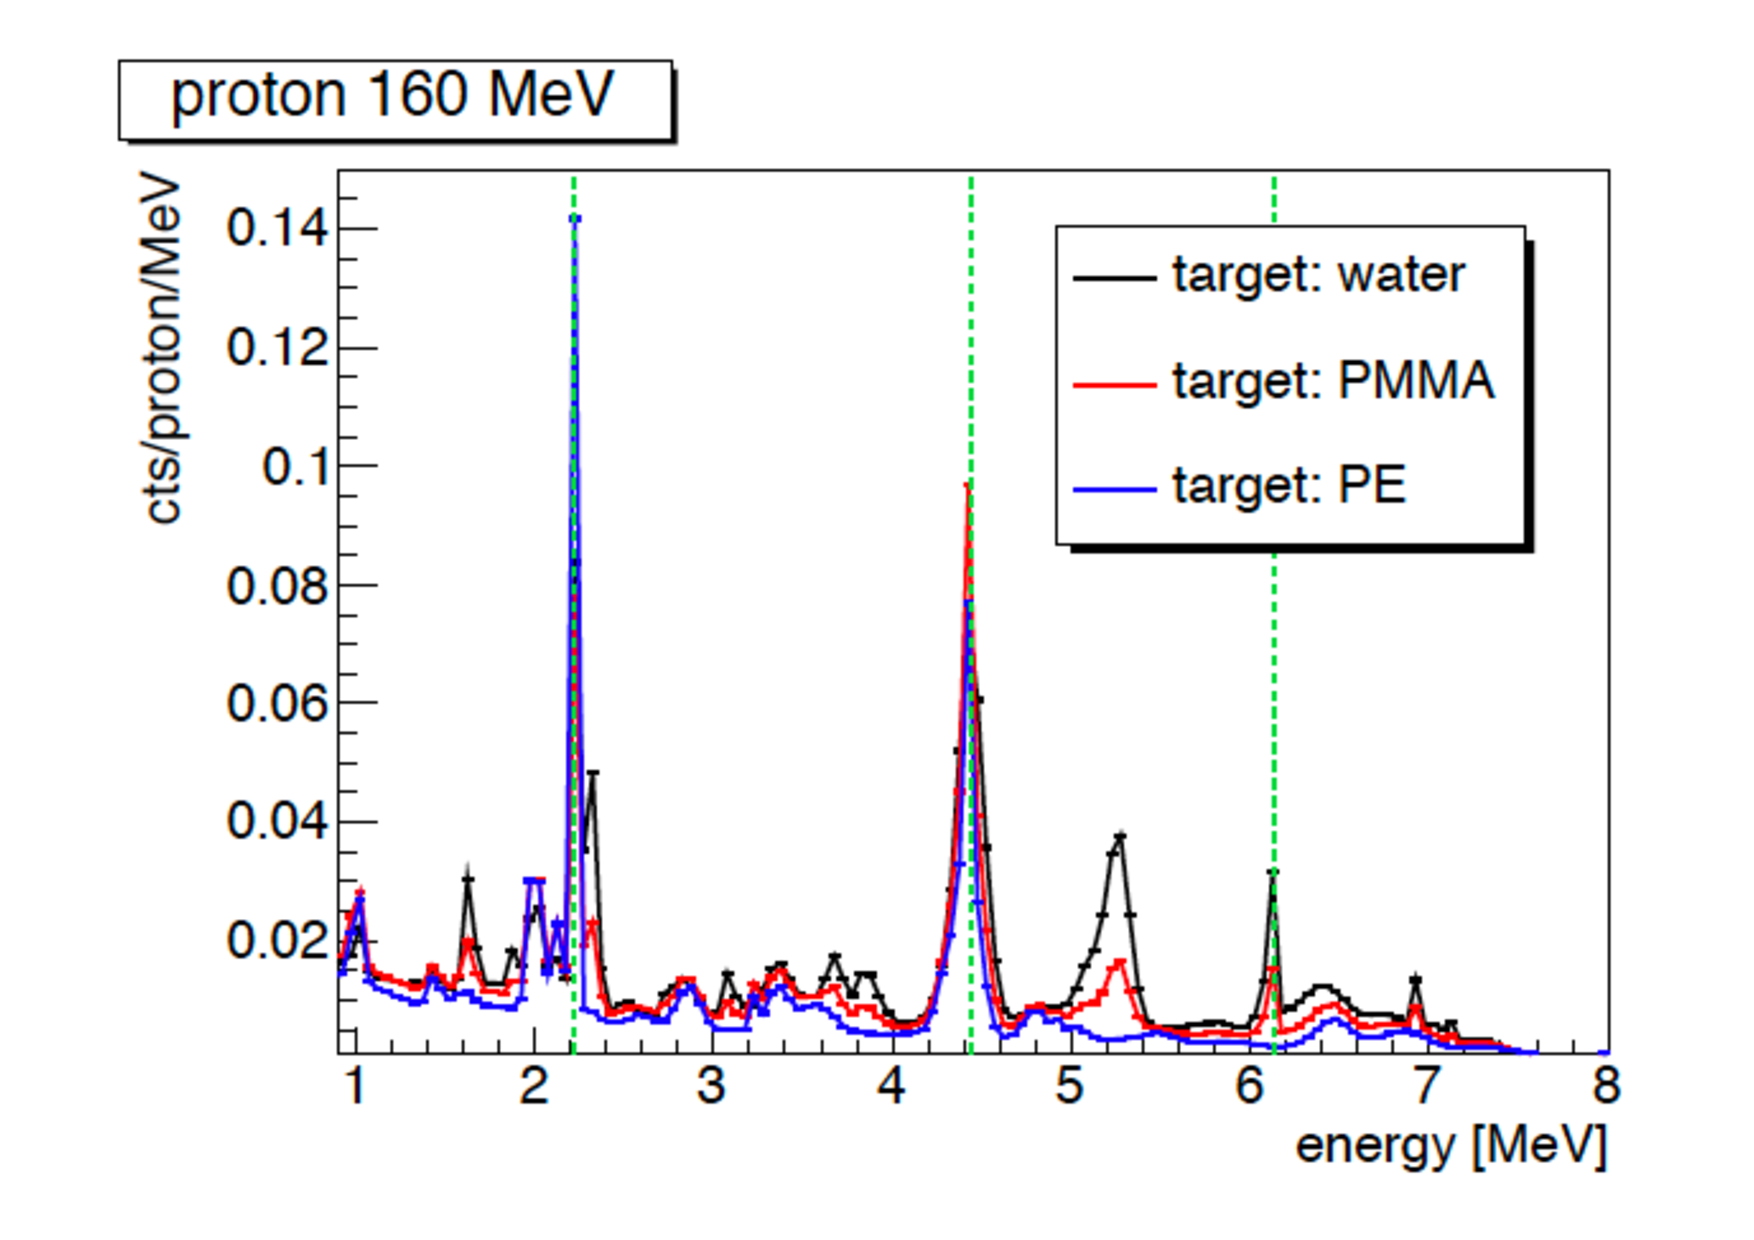
\includegraphics[width=1.\linewidth]{03_GraphicFiles/chapter2_GammaCameras/PG_E_targets.pdf}
\caption{\gls{pg} energy spectra resulting from the irradiation of \gls{pe}, \gls{pmma} and water targets (cylinders 15~cm diameter, 25~cm length) with 160~MeV protons. The vertical lines highlight specific spectroscopic transitions.}
\label{chap2::fig::PGEdistr}
\end{subfigure}
\begin{subfigure}[t]{.49\textwidth}
\hspace{-0.7cm}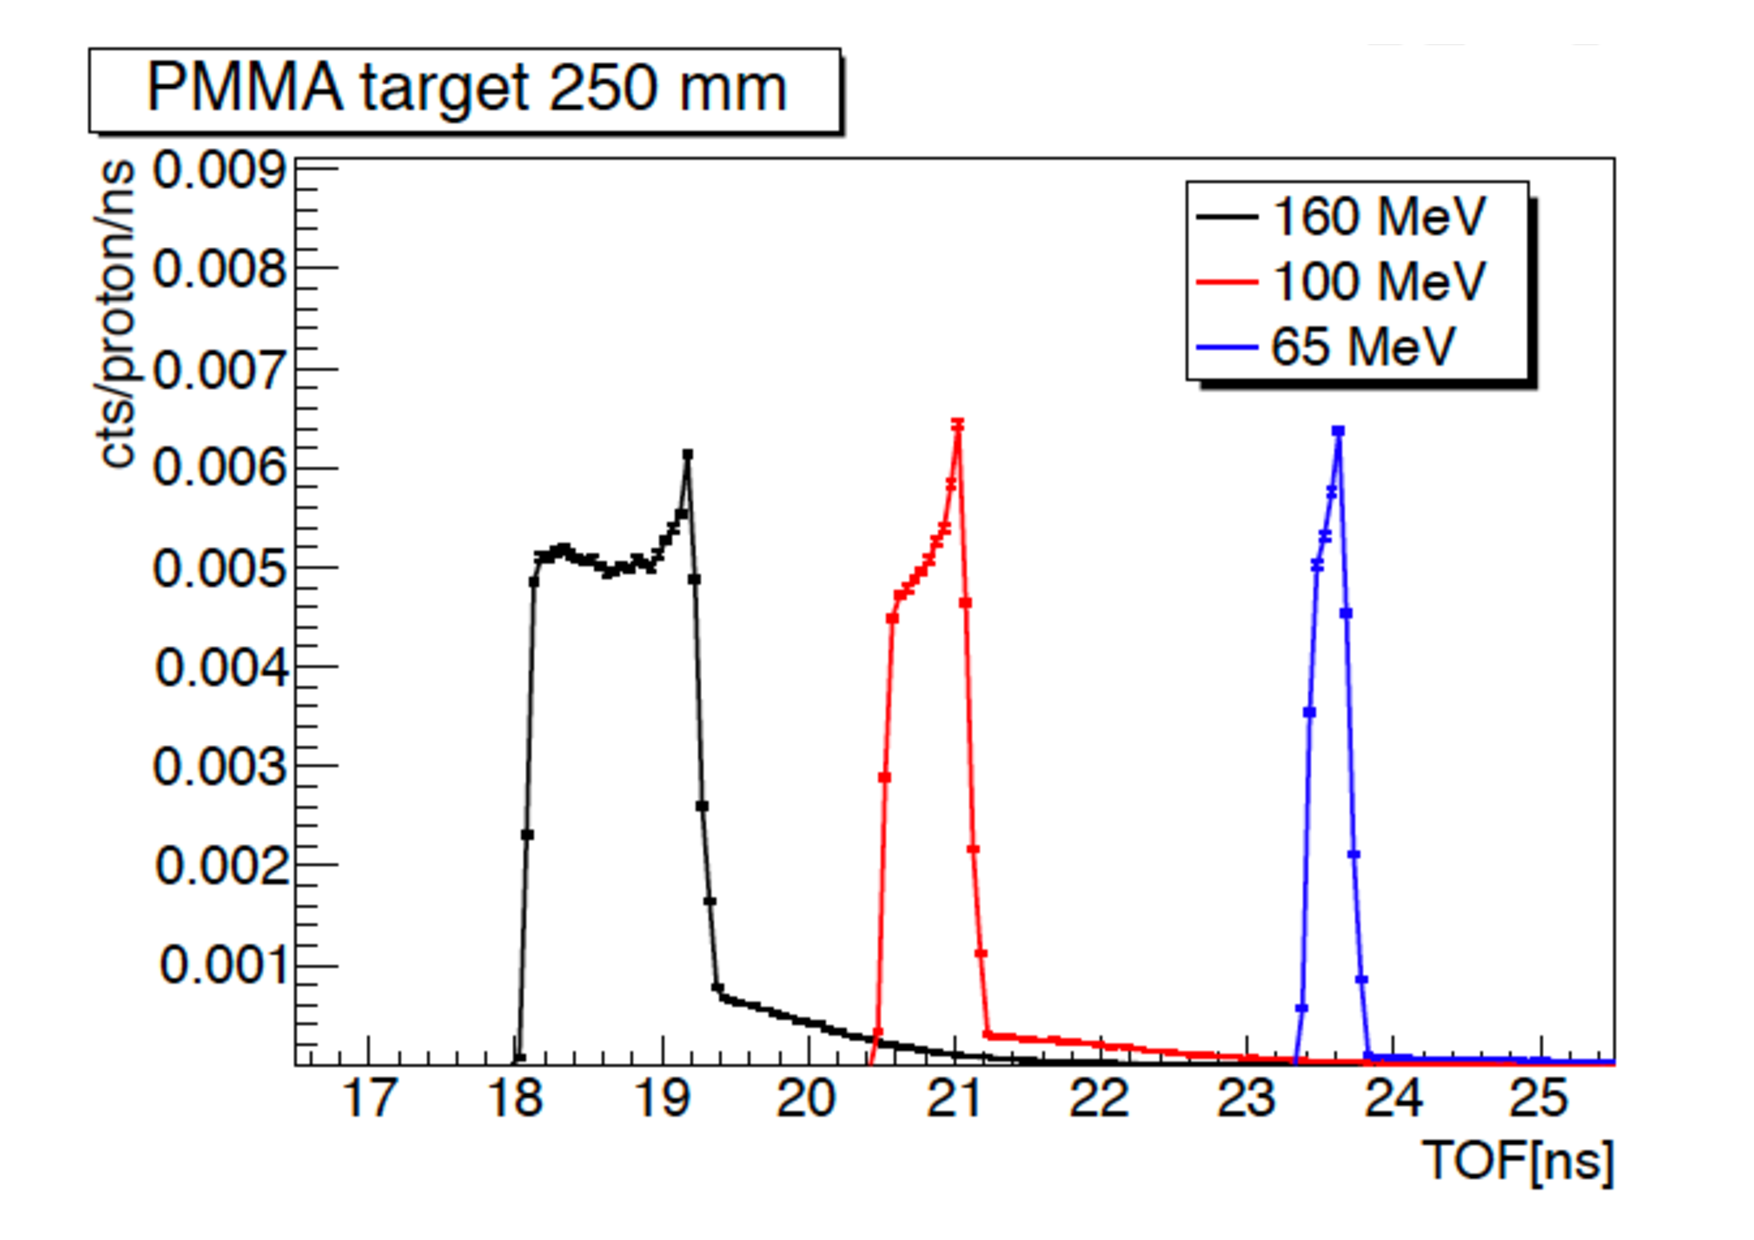
\includegraphics[width=1.\linewidth]{03_GraphicFiles/chapter2_GammaCameras/PG_TOF_PMMA.pdf}
\caption{\gls{tof} spectra of \glspl{pg} emerging from a \gls{pmma} cylindrical target (cylinders 15~cm diameter, 25~cm length) for 65~MeV, 100~MeV and 160~MeV proton beam irradiation.}
\label{chap2::fig::PGTdistr}
\end{subfigure}
\caption{In~\cite{Krimmer2017}.}
\label{chap2::fig::PG_ET}
\end{figure}

As mentioned, also time information can be used for range monitoring purpose. \myMarginnote{PG TOF distribution} \figurename~\ref{chap2::fig::PGTdistr} shows the \gls{tof} distribution of \glspl{pg} emerging from a \gls{pmma} target (15~cm diameter, 25~cm length) irradiated with 65~MeV, 100~MeV and 160~MeV proton beams. The influence of proton energy (range) on the spectrum peak position, width and integral is clear, and is the basic idea for two proposed monitoring techniques: \gls{pgt}, which is based on the \gls{tof} spectrum peak position and width~\parencite{Golnik2014}, and \gls{pgpi}, additionally exploiting the \gls{tof} spectrum integral to verify beam position and total dose, thus apporaching in vivo dosimetry~\parencite{Krimmer2017b}. 

All monitoring techniques based on \glspl{pg} must commonly deal with some specific \gls{pg} features. As a starting point, \gls{pg} production yields must be considered when designing monitoring prototypes. 
Specific measurements are needed for particle therapy, with peculiar beam energies, targets and irradiation fields, even if some data of \gls{pg} production by proton and carbon ions are available in the literature for general nuclear physics and astrophysics purposes~\parencite{Dyer1981, Kiener1998}.
In~\cite{Pinto2015} the authors studied the absolute \gls{pg} production yields in ten single-slit experiments with the irradiation of \gls{pmma} and water targets with proton and carbon ion beams, and the results are shown in \figurename~\ref{chap2::fig::PG_yields} for proton (left) and carbon ion beams (right) and summarized in table~\ref{chap2::tab::PG_yields_tab}, reproduced from the same publication. 

\begin{figure}
\centering
\begin{subfigure}[t]{.49\textwidth}
\hspace{-0.7cm}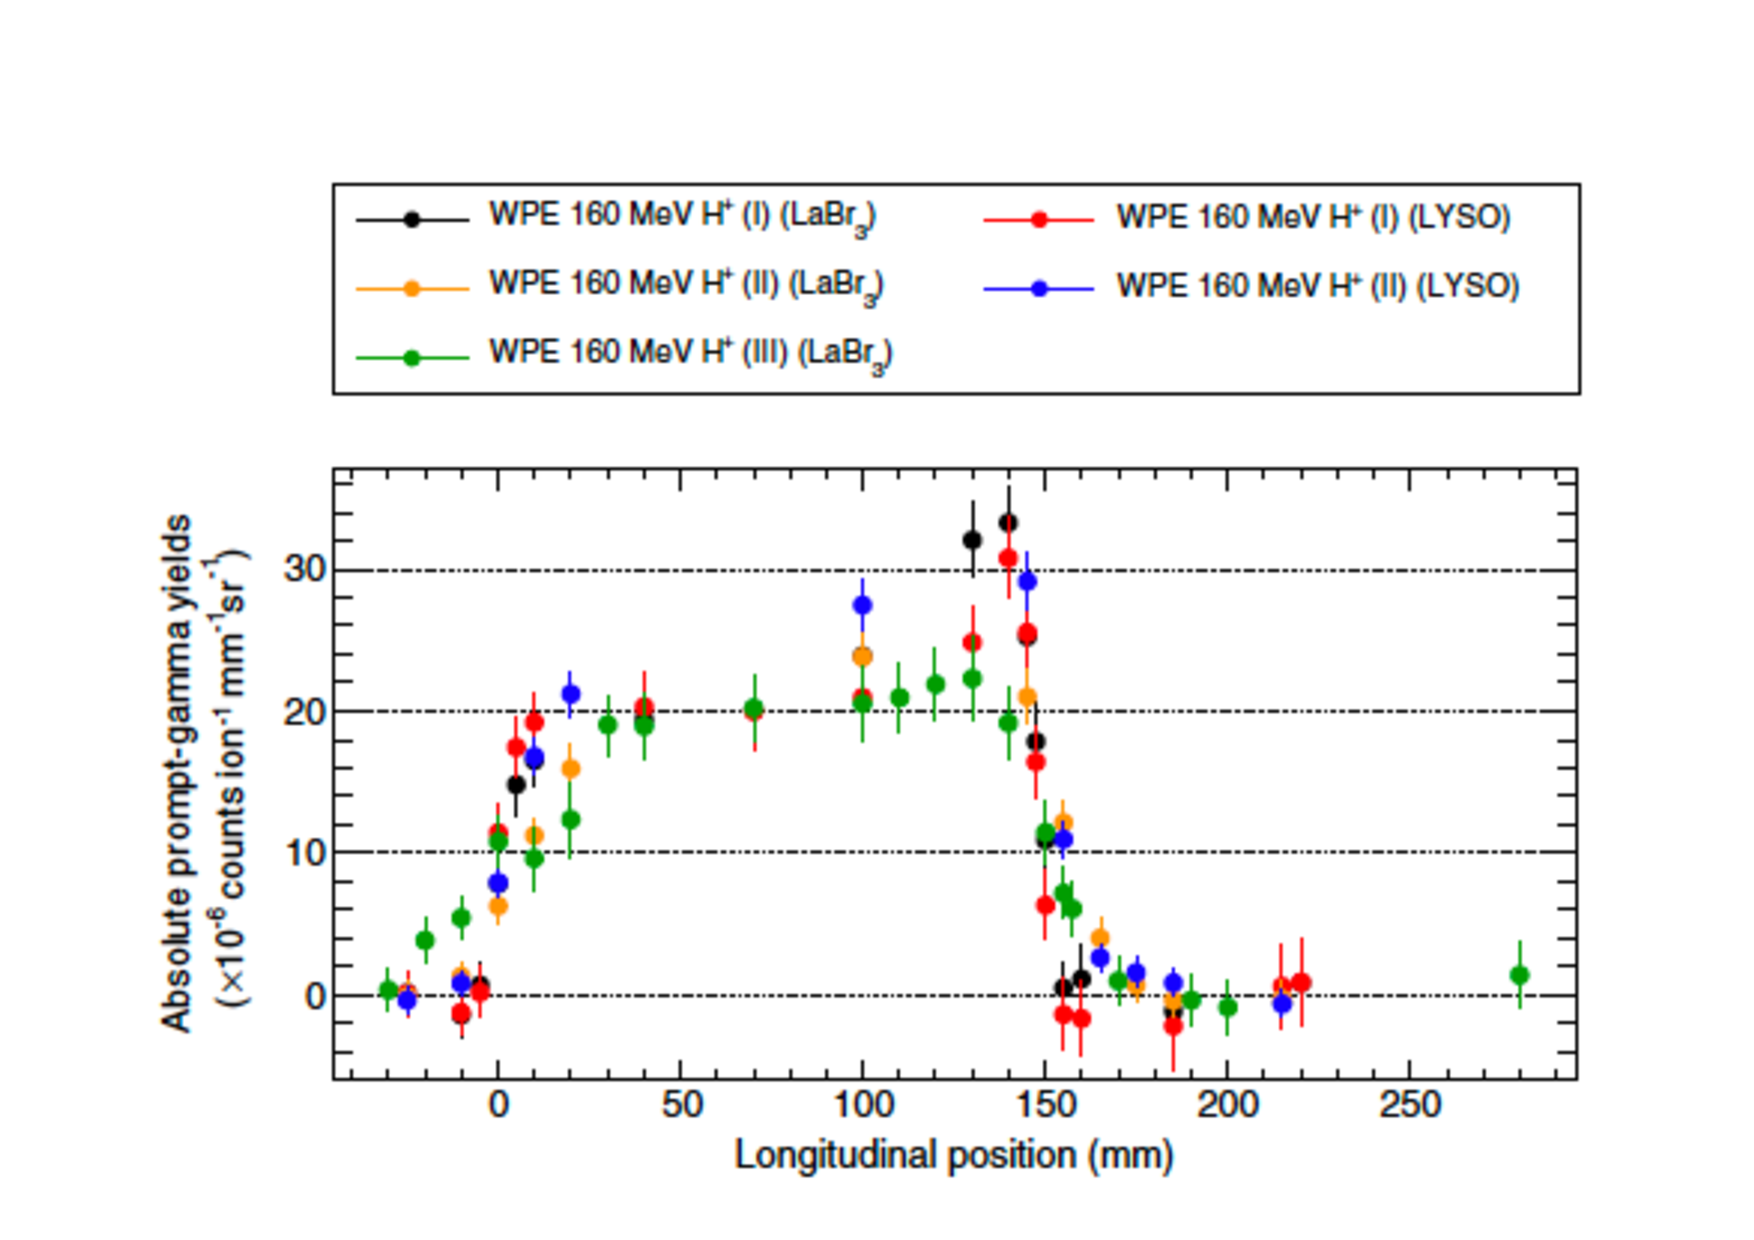
\includegraphics[width=1.2\linewidth]{03_GraphicFiles/chapter2_GammaCameras/PG_absYields_p.pdf}
\caption{Absolute \gls{pg} yields profiles for 160~MeV proton beam irradiation of a \gls{pmma} target. The different colors represent 5 different data sets, 3 obtained with \gls{labr3} detector, 2 with \gls{lyso} detector.}
\label{chap2::fig::PG_absYields_p}
\end{subfigure}
\begin{subfigure}[t]{.49\textwidth}
\hspace{-0.7cm}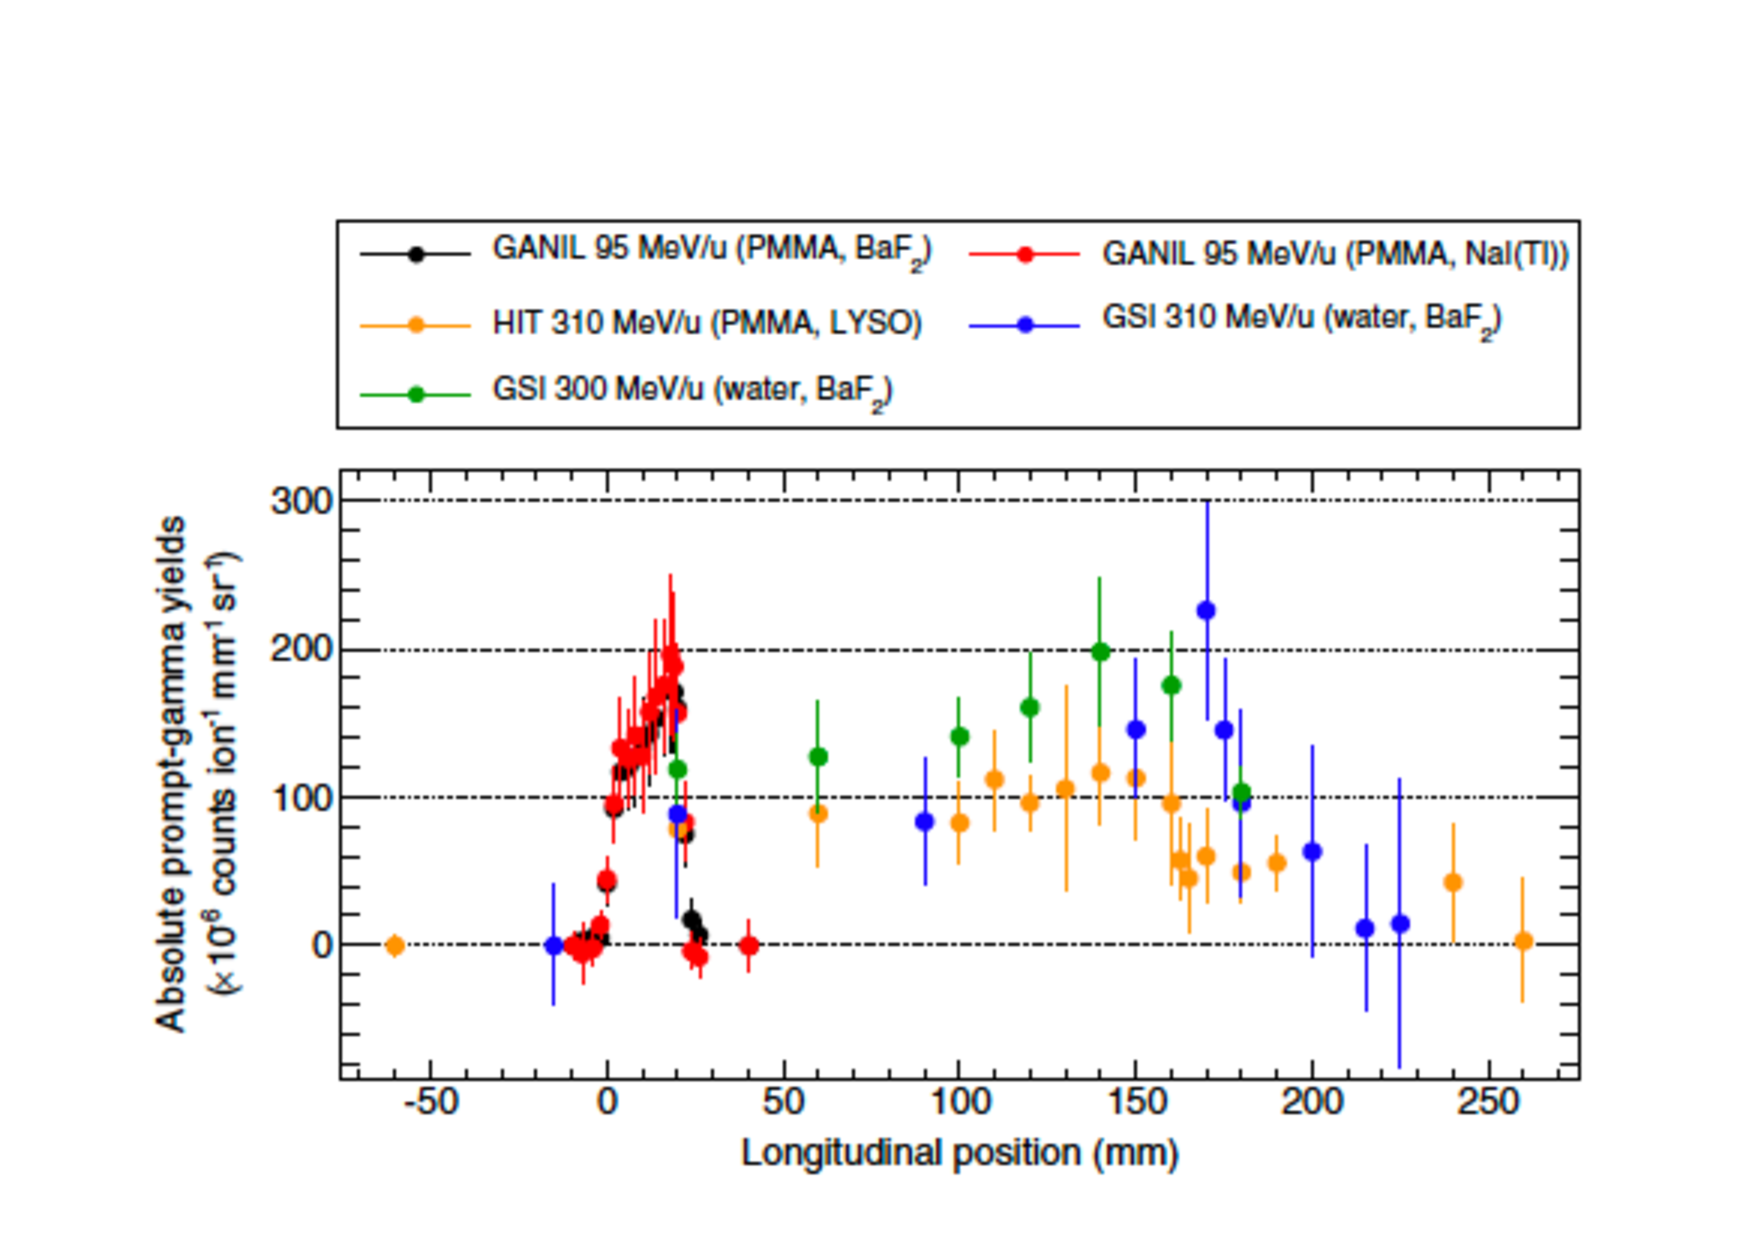
\includegraphics[width=1.2\linewidth]{03_GraphicFiles/chapter2_GammaCameras/PG_absYields_C.pdf}
\caption{Absolute \gls{pg} yields profiles for carbon ion beam irradiation of a \gls{pmma} target. The different colors represent 5 different data sets, collected at \gls{ganil}, \gls{hit} and \gls{gsi} with 95~MeV/u, 310 MeV/u adn 300~MeV/u carbon ion beams respectively. \gls{pmma} and water targets have been employed, and the \gls{pg} detection has been performed with \gls{baf2}, \gls{lyso} and gls{naitl} detectors.}
\label{chap2::fig::PG_absYields_C}
\end{subfigure}
\caption{In~\cite{Pinto2015}.}
\label{chap2::fig::PG_yields}
\end{figure}

\begin{table}[!htbp]
\centering
\caption{Absolute \gls{pg} yields measured in the first point after the \gls{pg} profile entrance rise. The energy range shows the energy range of the primary particles inside the \gls{fov} of the measurement point estimated in simulation. Table reproduced from~\cite{Pinto2015}.}
\label{chap2::tab::PG_yields_tab}
\resizebox{\textwidth}{!}{%
\begin{tabular}{llcc}
\toprule
\rowcolor{myColorMainA!20} 
\textbf{Material}& \textbf{Energy range (MeV/u)} & \textbf{Ion species} & \textbf{Absolute yield [$\times$10$^{-6}$ counts ion$^{-1}$mm$^{-1}$sr$^{-1}$]} \\
\midrule
\gls{pmma} & [77-90] & Carbon ions & 124 $\varpm$ 0.7 $_{\mathrm{stat}} \varpm$ 30 $_{\mathrm{sys}}$\\
\gls{pmma} & [272-310] & Carbon ions & 79 $\varpm$ 2 $_{\mathrm{stat}} \varpm$ 23 $_{\mathrm{sys}}$\\
Water          & [264-292] & Carbon ions & 112 $\varpm$ 1 $_{\mathrm{stat}} \varpm$ 22 $_{\mathrm{sys}}$\\
\gls{pmma} & [139-156] & Protons & 16 $\varpm$ 0.07 $_{\mathrm{stat}} \varpm$ 1 $_{\mathrm{sys}}$\\
\bottomrule
\end{tabular}}
\end{table}    

The comparison of \gls{pg} yields for proton and carbon ion beam irradiation with the same range in water, i.e. 160~MeV protons and 310~MeV/u carbon ions, shows a value approximately five times greater for the latter with respect to the former. Such an increased emission is due to the contribution of both projectile and target nuclei, while only the target nuclei can emit \glspl{pg} in proton irradiation. For carbon ions irradiation at different energies, an increased \gls{pg} emission has been verified for the lowest energy ions, as expected from published cross sections. Moreover, if comparing the \gls{pmma} and water targets for the same primary ion features, water results in an enhanced prompt photon emission. 
Other experimental results are reported in~\cite{Agodi2012, Agodi2013}: the authors measured \gls{pg} yields of 80~MeV/u carbon ions impinging on a \gls{pmma} target considering the full ion range, while in~\cite{Pinto2015} the results are normalized to the path length unit (1~mm). The found yield is (2.32$\varpm$0.01$_{\mathrm{stat}} \varpm$ 0.15 $_{\mathrm{sys}}$) $\times$ 10$^{-3}$ counts ion$^{-1}$sr$^{-1}$, which is compatible to the results in~\cite{Pinto2015} if the proper normalization is considered. Higher energy carbon ion beams (220~MeV/u) and \gls{pmma} targets have been employed to produce the results presented in~\cite{Mattei2015}. More recently, the same authors studied the prompt photon production of $^{4}$He, $^{12}$C and $^{16}$O beams interacting in \gls{pmma} target at \gls{hit}, showing good agreements with the aformentioned results (for carbon ions), and providing additional information about new ion species~\parencite{Mattei2017}. 
Furthermore, detailed information about specific \gls{pg} spectroscopic lines are reported in~\cite{Verburg2014, Verburg2013}, and have been recently published in~\cite{Kelleter2017}.

In order to resume the present knowledge about \gls{pg} production and give reference values for clinical applications, as reported in~\cite{Krimmer2017}, a rough estimate of the \gls{pg} yields per projectile for 15~cm range in water is 0.05 per proton and about 0.3 per carbon ion. These yields results to be similar to the one of the total amount of $\beta^{+}$ emitters~\parencite{Pinto2015, Robert2013}. However, Secondary radiation attenuation is another fundamental parameter to be considered, since only a fraction of the emitted photons will be able to emerge from the patient body and, at the same time, keep the information on the creation vertex. The higher energies of prompt photons (1-10~MeV) with respect to positron annihilation ones (511~keV) lead to an improved transmission through the patient body (factor 5), thus an increased expected detection rate~\parencite{Moteabbed2011}. 
The available \gls{pg} statistics for beam range monitoring can be assessed by considering the absolute yields measurements presented above (including attenuation considerations) and the average clinical beam intensities. In particular, 10$^{10}$ protons per second and 10$^{[7-8]}$ carbon ions per second are typical clinical values. For a monitoring on a single spot basis, which is highly desirable, the most important spot (generally in the distal region of the \gls{ptv}) can be chosen as reference: the number of incident ions in such a spot is approximately 10$^8$ and $10^6$ for protons and carbon ions, respectively~\parencite{Kramer2000, Grevillot2012}. For these kinds of spots, in the whole solid angle, about 10$^7$ (for protons) and 10$^5$ (for carbon ions) \gls{pg} rays are emitted in the spot duration. This number is then reduced by the detection device efficiency and \gls{fov}. 

\subsection{Simulation of prompt-gamma emission and detection}\label{chap2::subsec::PGsimulation}

The general objective of \gls{pg} control of particle therapy treatment is the ion range on-line monitoring, which is performed via a comparison between measured and predicted \gls{pg} distributions, in accordance with the treatment planning. The prediction of \gls{pg} emission profiles relies on simulations, which are based on the experimental data described in the previous paragraph, and must include the prediction of the detector response. Precision and accuracy of the physical models and the reference data are crucial in the simulation process, also given the complex dependency of \gls{pg} yields to parameters such as beam features (ion species, energy, spatial distribution) and target composition. 

Monte Carlo simulation approaches are generally time consuming~\parencite{Robert2013, Dedes2015, Schumann2015}, and several approaches are being studied to reduce the calculation time and allow for direct translation to clinics. \gls{gpu}-oriented implementations highly improves the simulation efficiency, and some solutions have been successfully tested. Clinically acceptable dose calculation accuracy has been achieved with few tens of seconds of calculation time required, but electron and neutron transport have been disabled in the code described in~\cite{Qin2017}. With respect to standard Monte Carlo codes, an improvement in efficiency of three orders of magnitude is reported for the clinical validation of the code gPMC (\gls{gpu}-based \gls{mc} code for proton dose calculation ) in~\cite{Giantsoudi2015}. 
Alternative approximate methods are based on the \gls{vrt}, already implemented, for example, for in-beam \gls{pet} predictions~\parencite{Sommerer2009}. It has been shown that computation time can be reduced by about three orders of magnitude for the prediction of full three-dimensional \gls{pg} maps with respect to standard \gls{mc} codes~\parencite{Huismann2016, ElKanawati2015}. The calculation can be achieved in about two hours on a single core computer; this makes the clinical implementation possible, even if further improvements are still needed.  
As a general remark, it must be noticed that \gls{mc} tool-kits have not been conceived for the energy range of interest in particle therapy, thus a fine tuning of the model parameters is necessary. The comparison of different \gls{mc} codes often results in large differences in the \gls{pg} simulated yields~\parencite{Bohlen2010, Verburg2012, Schumann2015}, and the hadronic models still have to be improved, ideally with the availability of differential cross-sections and \gls{pg} yields further measurements in the clinical energy range~\parencite{Newhauser2015}. However, substantial enhancement have been achieved in the \gls{qmd} model~\parencite{Dedes2014}, and quantitative characterization of \gls{pg} emission yields have been performed~\parencite{Schumann2015, Pinto2016}.

In addition to \gls{mc}-based approaches, also the implementation of analytic models is efficient~\parencite{Sterpin2015, Russo2016}, even if they are based on pre-computed \gls{pg} profiles obtained with \gls{mc} calculations, thus they suffer from the aforementioned uncertainties.
Finally, the pre-computation of \gls{pg} profiles is not required by filtering approaches, which make use of the dose distribution maps, available form the treatment planning, and directly get the expected \gls{pg} distribution~\parencite{Kroniger2015}.  
  
\section{PG ion range monitoring devices: state of the art}\label{chap2::sec::PGdevices}

The detection of \gls{pg} rays for particle therapy monitoring has been proposed already in 2003~\parencite{Stichelbaut2003}, and since then several approaches have been investigated by developing adapted detection devices. The specificity of particle therapy range control techniques based on \glspl{pg} requires the design of dedicated detectors, adapted to a wide photon energy spectrum and able to cope with the background level expected during particle therapy treatments. Standard medical imaging cameras, like the Anger cameras employed for \gls{spect} examinations, cannot be adapted to such requirements. 
The explored solutions to create clinical prototypes can be classified, as proposed in~\cite{Krimmer2017} and already mentioned in this chapter, in imaging devices, based on the spatial information provided by each collected prompt photon, and non-imaging ones, which exploit integrated prompt photon yields. In table~\ref{chap2::tab::PGmodalities_tab}, reproduced from~\cite{Krimmer2017}, the main features exploited by the developed modalities are summarized.

\begin{table}[!htbp]
\centering
\caption{Characteristics of the \gls{pg} monitoring modalities. The star symbol represents mandatory measurements, the star in brackets means auxiliary but not mandatory measurements. Table reproduced from~\cite{Krimmer2017}.}
\label{chap2::tab::PGmodalities_tab}
\resizebox{\textwidth}{!}{%
\begin{tabular}{l | ccccc}
\toprule
\rowcolor{myColorMainA!20} 
\textbf{PG} & \multicolumn{2}{c}{\textbf{Imaging systems}} & \multicolumn{3}{c}{\textbf{Non-imaging systems}} \\ 
%\rowcolor{myColorMainA!20} 
%\cmidrule(lr){2-3}\cmidrule(lr){4-6}
\rowcolor{myColorMainA!20} 
 \textbf{features}   & Physical & Electronic & PG timing & PG peak integral & PG spectroscpy\\
\rowcolor{myColorMainA!20} 
    & collimation & collimation & (PGT) & (PGPI) & (PGS)\\    
\midrule
Position & $\star$ & $\star$&  & &  \\
Energy & ($\star$) & ($\star$) & ($\star$) &  ($\star$) & $\star$\\
TOF & ($\star$) & ($\star$) & $\star$& $\star$& ($\star$) \\
\bottomrule
\end{tabular}}
\end{table}      

In the following sections, the state of the art of the various \gls{pg} monitoring modalities is present following the proposed classification.

\subsection{Non-imaging prototypes}\label{chap2::subsec::PGdevices_nonImaging}

Non-imaging \gls{pg} monitoring solutions are based on the integrated measurement of time or energy resolved photon spectra, and exploit the indirect relation between the characteristics of such spectra and the primary ion range to verify the conformity of the delivered treatment to the planned one. The objective of such techniques is not to retrieve spatial information from the collected photons, thus less demanding detectors are required with respect to imaging solutions, and the footprint in the treatment room is minimized, as well as the device cost. 

As the primary ion beams interacting in the patient during treatments \myMarginnote{PGT} cause nuclear excitation and, thus, the emission of prompt photons along their path, until they are stopped, the total transit time depends on the total ion range. The width of the \gls{pg}-\gls{tof} spectrum can be then correlated to the ion range. Such a monitoring method has been first proposed in 2014 by Golnik and colleagues~\parencite{Golnik2014} and tested with 150~MeV protons at the AGOR cyclotron, KVI-CART. The proton beam irradiated a homogeneous graphite target (10$\times$10$\times$30~cm$^3$, density 1.7~g~cm$^{-3}$), with an expected range of 10.3~cm; the target has been set in three different positions (20~mm between each position), and the gamma detection has been performed with a \gls{gaggce} cylindrical detector.  The setup is shown on the left side of \figurename~\ref{chap2::fig::PGT_shifts}, and the resulting spectra are shown  on the right side.

\begin{figure}[!htbp]
\centering
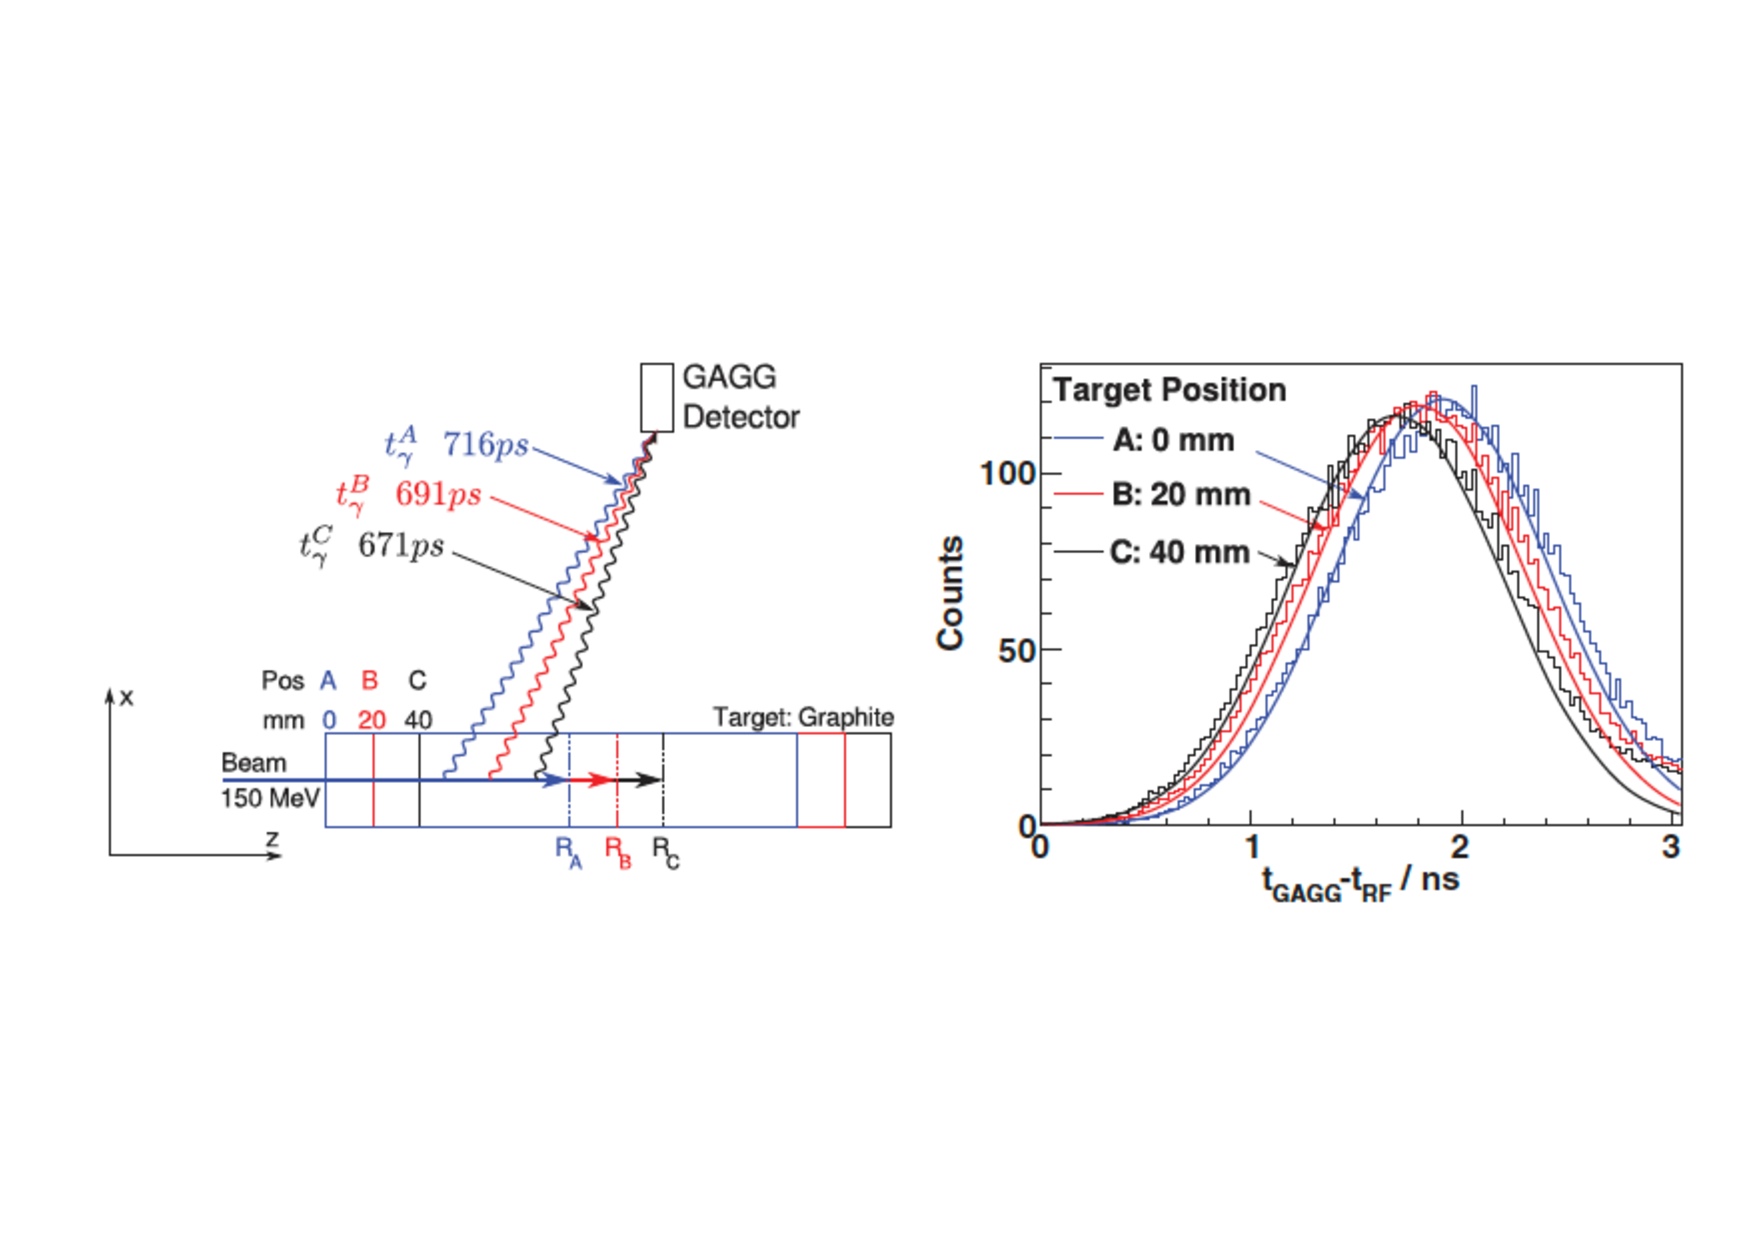
\includegraphics[width=0.8\textwidth]{03_GraphicFiles/chapter2_GammaCameras/PGT_shifts.pdf}
\caption{(Left) Setup for the irradiation of a graphite target with 150~MeV proton beams. The target was set in three different positions, with successive 20~mm shifts. (RIght) Resulting \gls{pg}-\gls{tof} spectra; the photon measurements has been performed with a \gls{gaggce} cylindrical detector. The experimental data are normalized to 10$^9$ incident protons. In~\cite{Golnik2014}.}
\label{chap2::fig::PGT_shifts}
\end{figure}  

The shift of the average spectrum position, corresponding to the target shift, is clearly visible.In the same work, the authors also present the results of the irradiation with the same proton beam (150~MeV) of \gls{pmma} target at increasing thickness, from 5 to 15~cm. The detection has been performed with the same \gls{gaggce} detector. The resulting \gls{tof} spectra are shown in \figurename~\ref{chap2::fig::PGT_PMMA}.

\begin{figure}[!htbp]
\centering
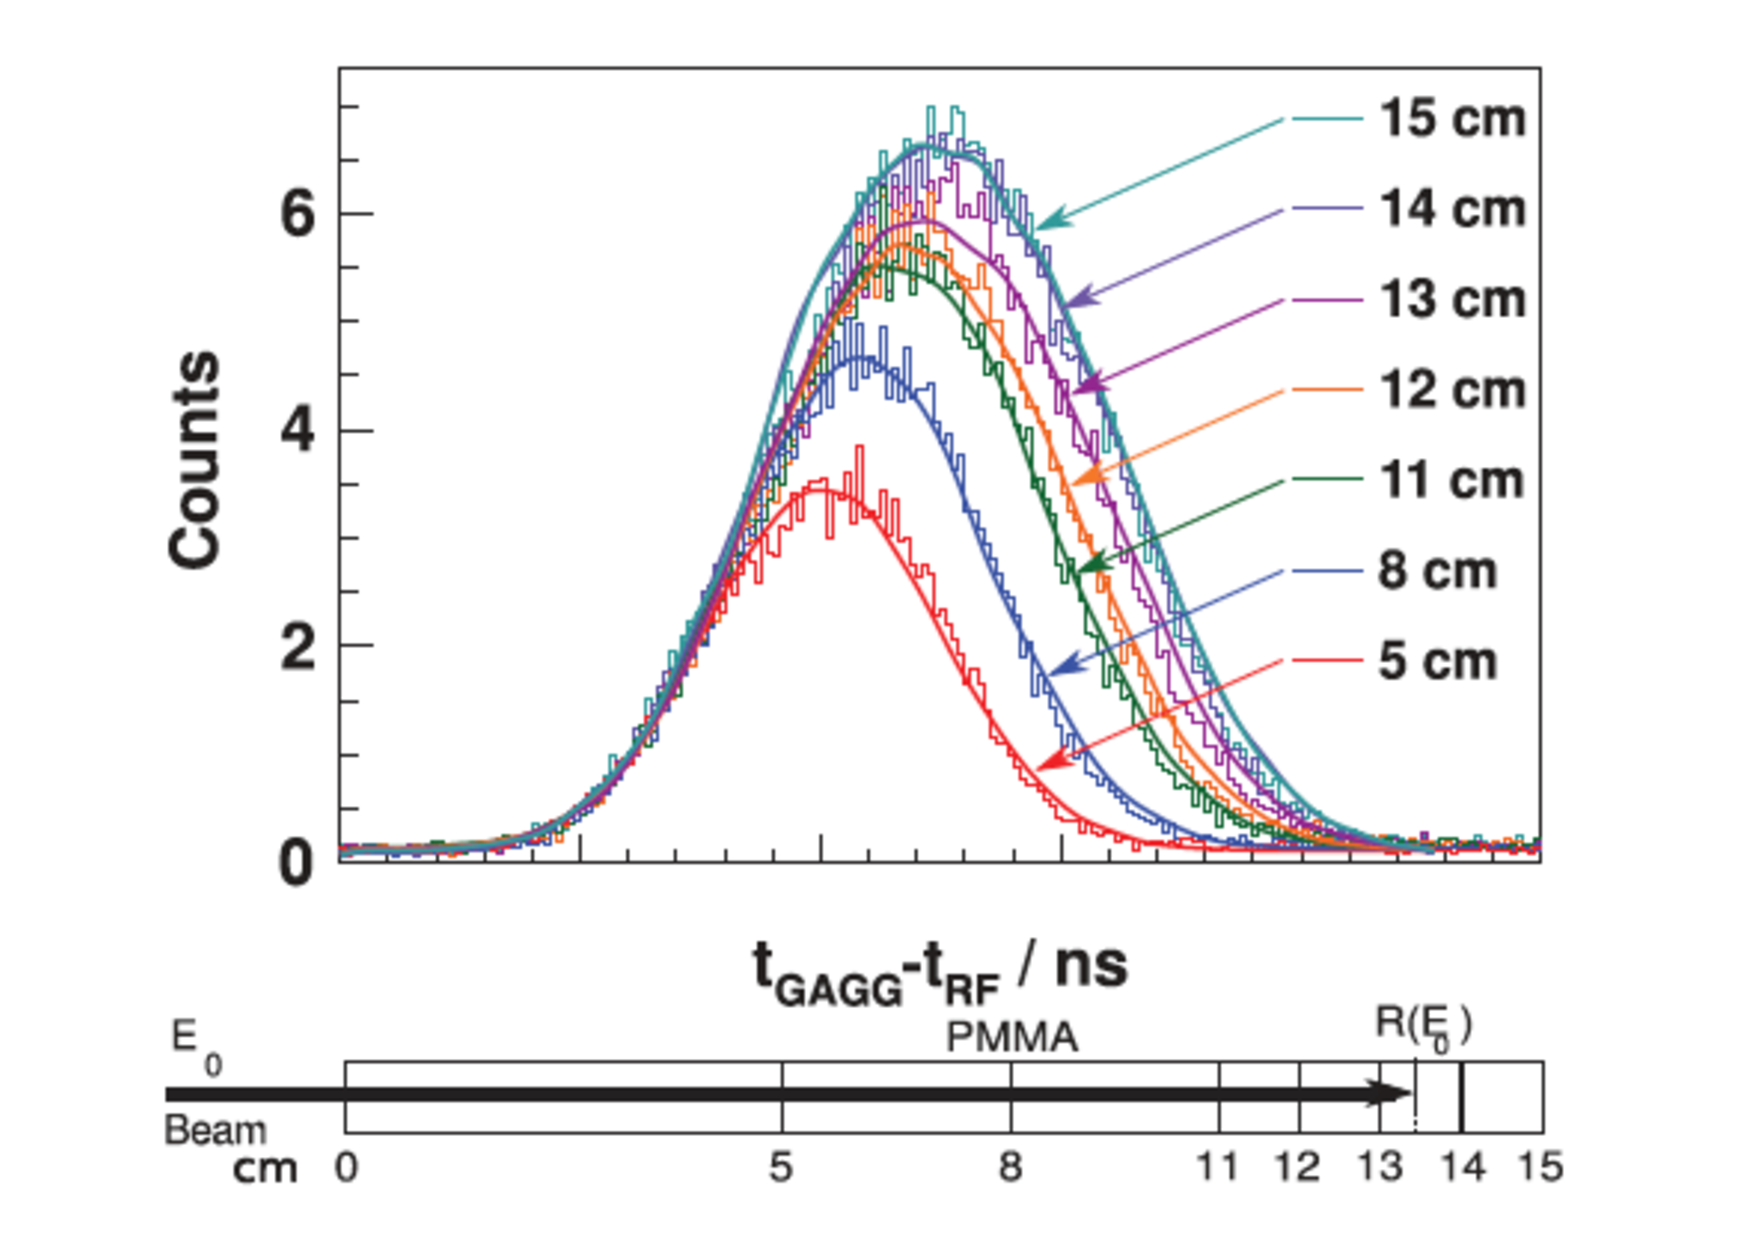
\includegraphics[width=0.8\textwidth]{03_GraphicFiles/chapter2_GammaCameras/PGT_PMMA.pdf}
\caption{Comparison of simulated and experimental \gls{pg}-\gls{tof} profiles obtained with the irradiation of \gls{pmma} targets with increasing thickness. The \gls{pg} detection is performed with a \gls{gaggce} detector. In~\cite{Golnik2014}.}
\label{chap2::fig::PGT_PMMA}
\end{figure}  

The beam expected range was 13.6~cm, so that it stopped in the target only for 14 and 15~cm thick \gls{pmma} blocks. \figurename~\ref{chap2::fig::PGT_PMMA} shows the good agreement between simulated (solid lines) and experimental data (histograms), and the shift and broadening of the \gls{pg}-\gls{tof} spectra with the increasing target thickness. Similar results have been also obtained by simulating proton beams at increasing energies, from 50 to 230~MeV, corresponding to a range change in the range [2-17]~cm. Simulation studies also included the irradiation of heterogeneous targets, and the experimental clinical verification was performed at the proton treatment center in Essen, equipped with an \gls{iba} C230 cyclotron, with several phantoms and detectors. The range variations in a stacked \gls{pmma} target, as well as the effect of air cavities and bone inserts have been verified, and the \gls{pgt}-based range verification showed the ability to detect 5~mm range shifts in heterogeneous targets for clinical relevant doses, but the strong influence of the accelerator \gls{rf} signal stability has also been highlighted~\parencite{HuesoGonzalez2015b}. The \gls{tof} measurement was actually based on the accelerator \gls{rf} signal, and a phase variation on the time-scale of hours caused shifts in the \gls{tof} spectrum equivalent to the one provoked by the shift of the target of a few centimeters. The author pointed out the need of a beam monitoring system to provide the time reference for the \gls{tof} measurement; such a beam monitor has been developed and tested to characterize the bunch structure of the clinical C230 cyclotron of the Oncoray center in Dresden~\parencite{Petzoldt2016}. 
In \figurename~\ref{chap2::fig::PGT_stats} the authors show the ability of this monitoring method to detect range shifts due to target in-homogeneity for decreasing amount of primary protons: shifts due to bone and air inserts in an homogeneous \gls{pmma} can be detected for primary statistics down to 10$^8$ primary protons, with increasing uncertainty for decreasing number of primaries.  

\begin{figure}[!htbp]
\centering
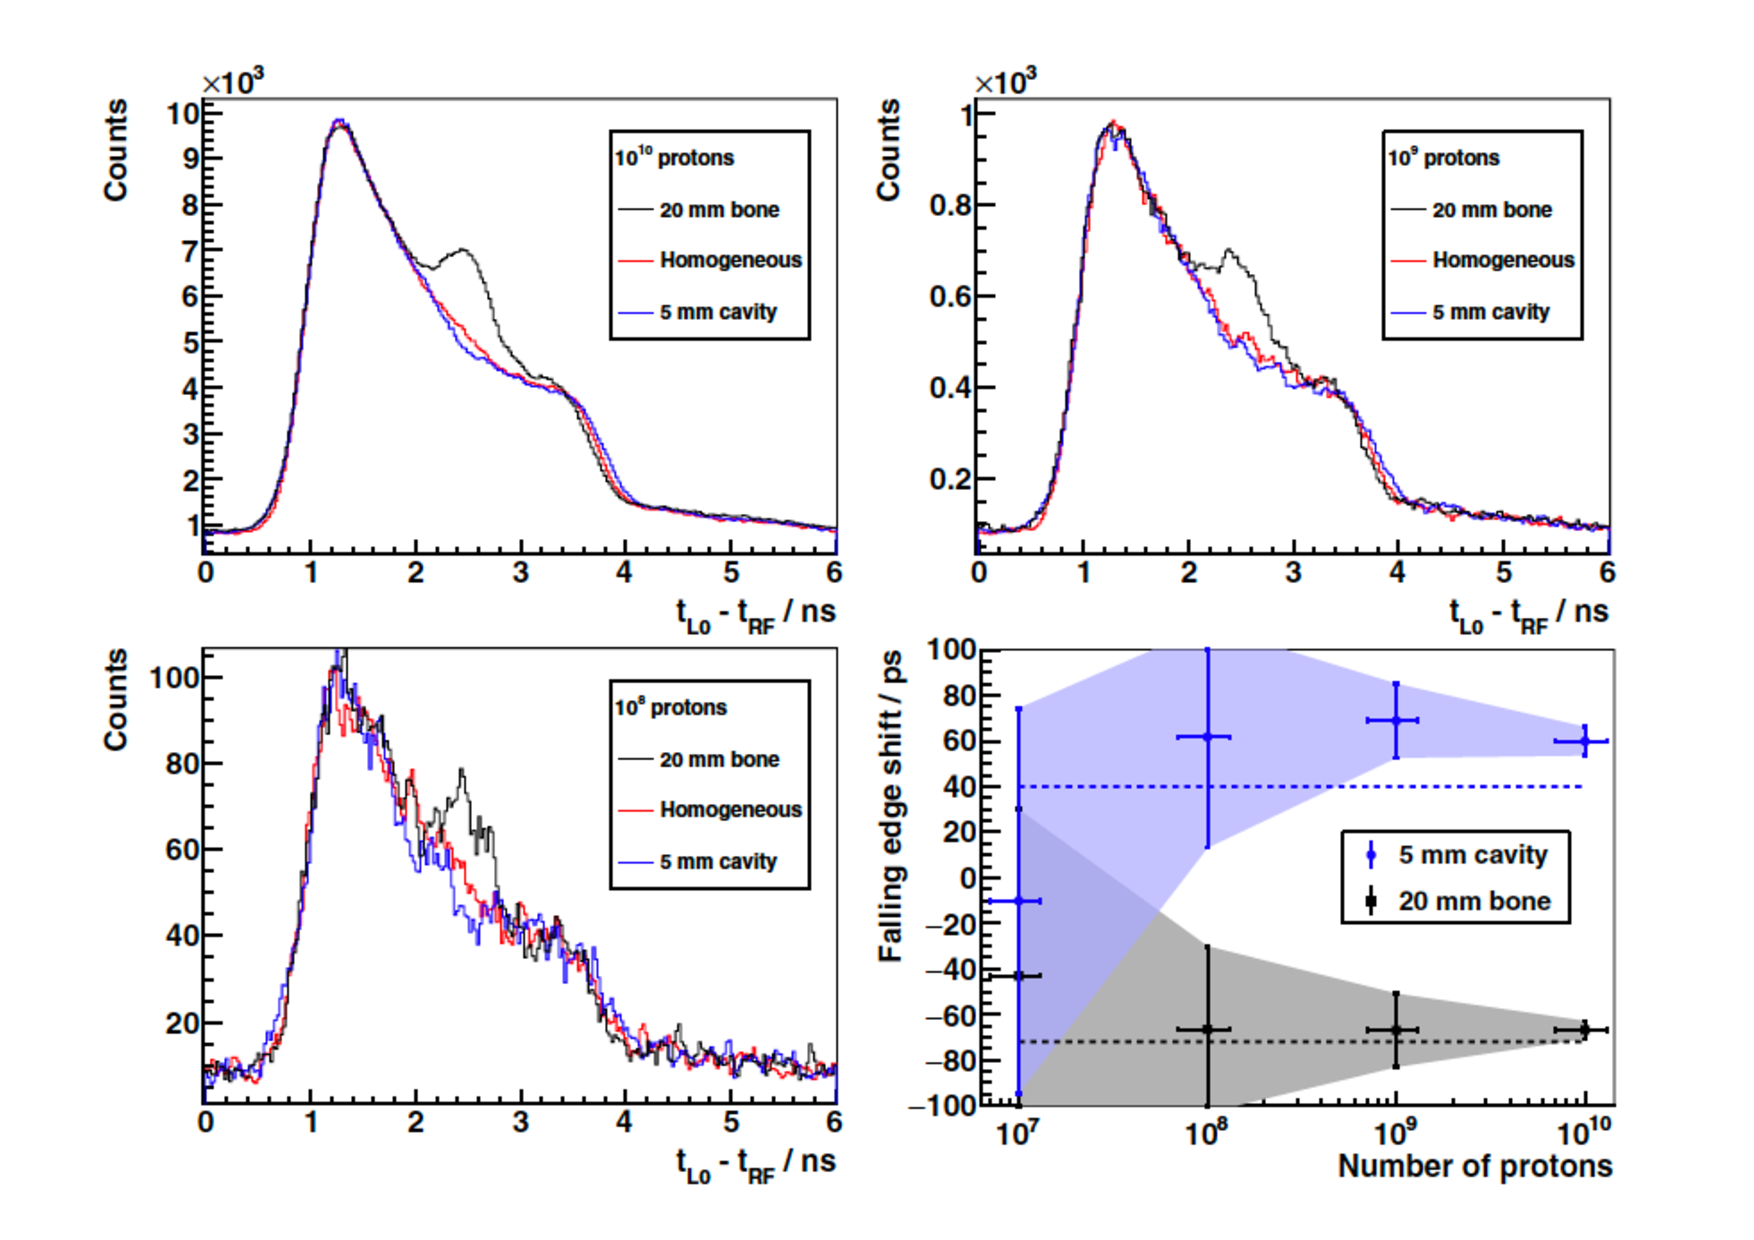
\includegraphics[width=0.8\textwidth]{03_GraphicFiles/chapter2_GammaCameras/PGT_stats.pdf}
\caption{First three panels: \gls{pg}\gls{tof} spectra obtained with the 230~MeV proton irradiation of an homogeneous \gls{pmma} target and two targets with air and bone inserts are compared for increasing number of primary protons. The \gls{pg} detection is performed with an \gls{labr3} detector (L0). The bottom right panel shows the shift of the spectra falling edge with respect to the homogeneous target case as a function of the number of incident protons. In~\cite{HuesoGonzalez2015b}.}
\label{chap2::fig::PGT_stats}
\end{figure}  

It has been estimated in~\cite{Pausch2016} that 10$^4$ detected \gls{pg} rays are needed to reveal a 5~mm range shift, with a bunch width of 2~ns.This is a fundamental requirement to be taken into account when designing a prototype for this application, together with the expected data throughput, which is significant given the absence of collimation system. However, with energy selected gamma rays of several MeV, a timing resolution of 200~ps have been obtained with optimized detector configurations, and throughput rates of about 600 kcps (kilo counts per second) have been handled~\cite{Pausch2016}. 

The time resolved measurement of \gls{pg} rays is also exploited in the \gls{pgpi} monitoring method. The integral of the \gls{pg} peak in the \gls{tof} spectrum measured with various detectors located at different positions around the target is used to control the ion range. \myMarginnote{PGPI} After preliminary studies at the in Arronax cyclotron in Nantes, experimental tests have been performed at the \gls{cal} in Nice, following previous results published in~\cite{Carnicer2012} and obtained with the same accelerator. 65~MeV protons at an intensity of 3$\times$10$^9$ protons per second have been used to irradiate an homogeneous \gls{pmma} target, and the \gls{pg} rays have been collected with \gls{labr3} scintillators read-out with a dedicated card developed at the \gls{ipnl}. The accelerator \gls{rf} signal or a beam monitoring system have to be used to provide the time reference for the \gls{tof} measurement. For this first study, the data have been synchronized to the positions of the modulator wheel used for passive beam delivery, provided via a photosensor. In \figurename~\ref{PGPI_spectra} the \gls{pg} spectra collected for two different positions of the modulator (corresponding to the maximum thickness and the hole) are shown~\parencite{Krimmer2017b}. The integral is calculated after background subtraction and the selection of the \gls{tof} proper window for the \gls{pg} selection, and compared for different detectors in various positions. The ratios of the integrals measured in different positions are able to show few percent variations in the \gls{pg} emission rate, corresponding to few millimeter range deviations, with simple and quick analytic data processing.

\begin{figure}[!htbp]
\centering
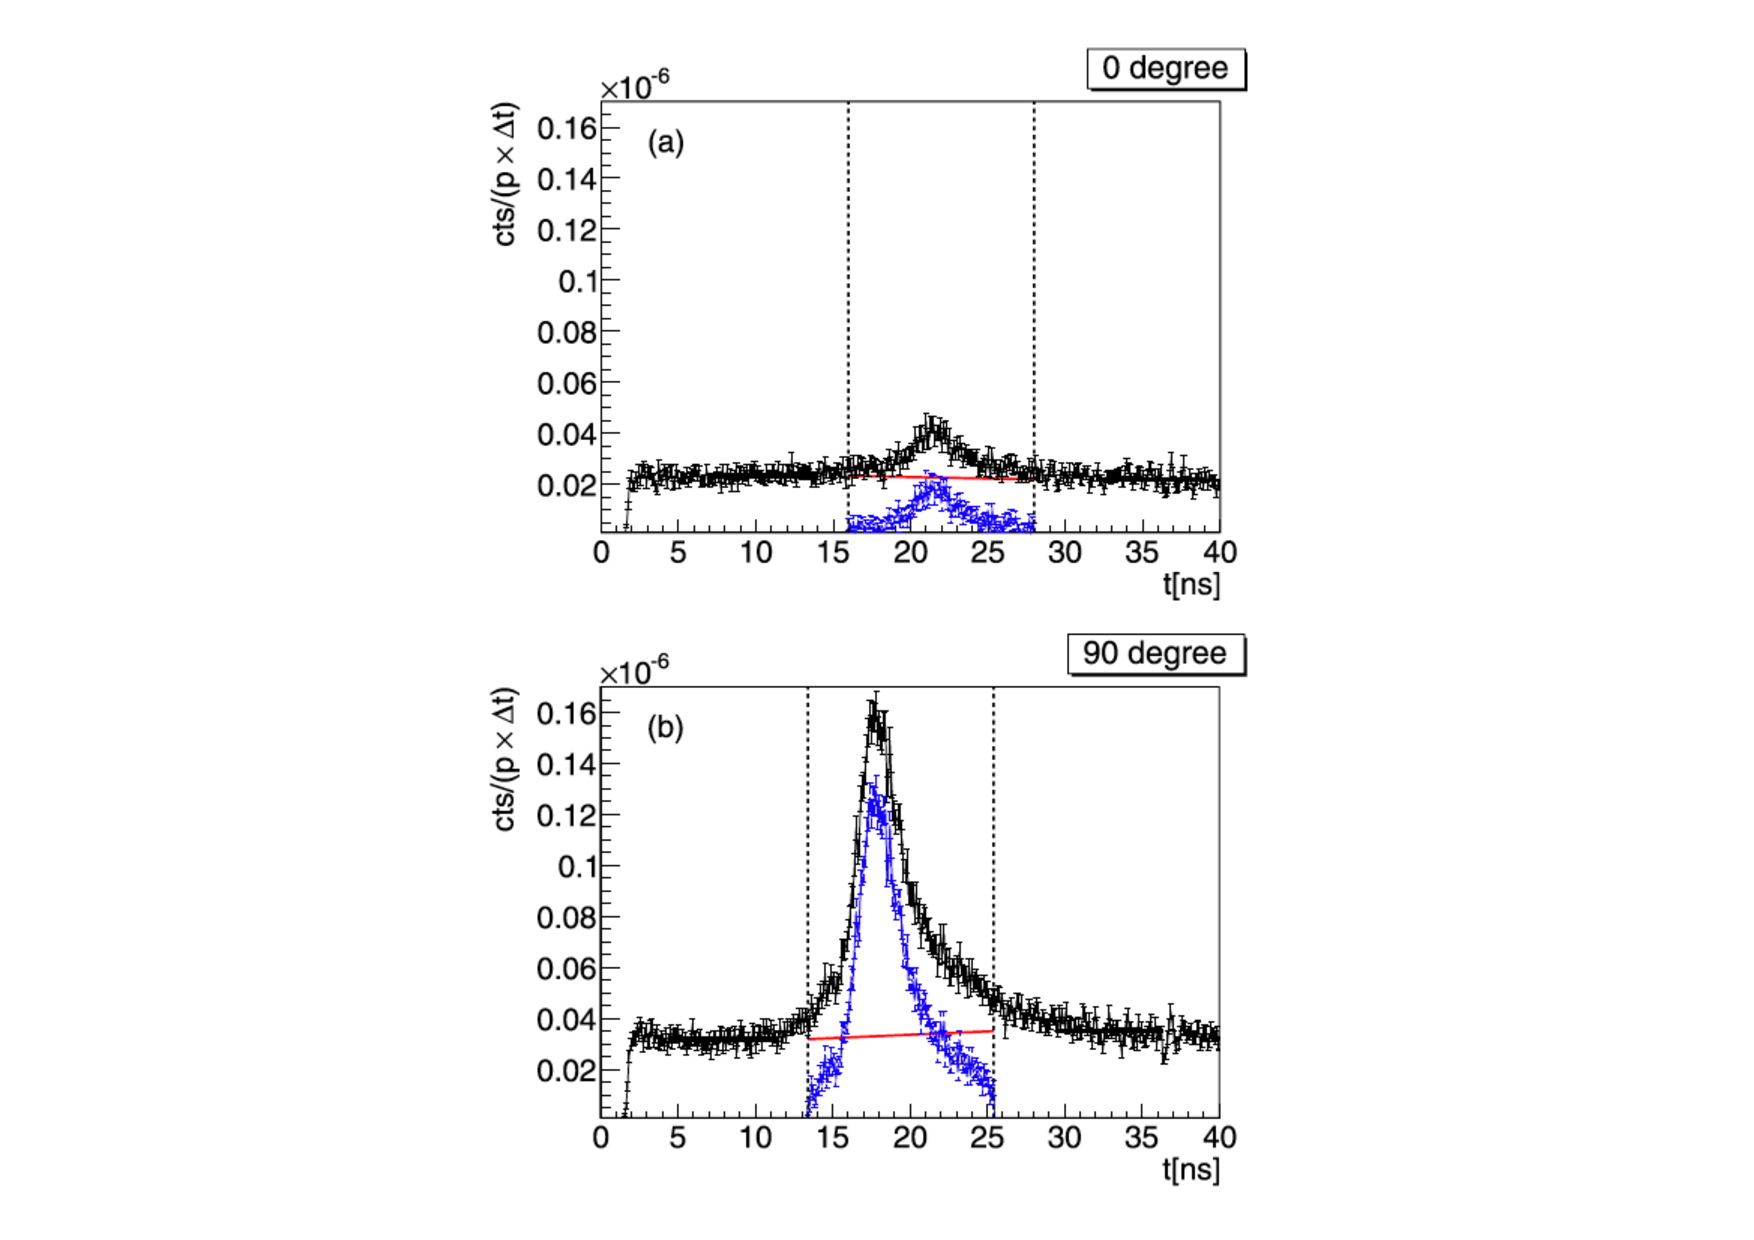
\includegraphics[width=0.8\textwidth]{03_GraphicFiles/chapter2_GammaCameras/PGPI_spectra.pdf}
\caption{\gls{tof} spectra measured for two positions of the modulator wheel, corresponding to the maximum thickness (0\textdegree) amd the hole (90\textdegree). An energy threshold of 1~MeV have been applied for the gamma detection. After background subtraction (red line), the integral is calculated in the range delimited by the vertical dashed lines. In~\cite{Krimmer2017}.}
\label{chap2::fig::PGPI_spectra}
\end{figure}  

In the case of 65~MeV protons, such a method has been verified to be able to detect 3~mm range shifts in \gls{pmma}. In addition, the authors also highlight that absorption in the target can determine similar effects on the \gls{pg} spectra, so that with the combination of signals from several detectors placed around the target, its position can be retrieved~\parencite{Krimmer2017b}.

As an alternative to time resolved measurements, energy resolved \gls{pg} spectra can provide indirect information\myMarginnote{PGS} about the ion range in matter through the direct estimate of the target composition.


\parencite{Verburg2012, Verburg2013, Verburg2014, Testa2014, Verburg2015, Polf2009, Polf2009b, Polf2013} 57-82-21-144-145-146-147-148

\subsection{Imaging prototypes}\label{chap2::subsec::PGdevices_Imaging}



LINE CONE RECONSTRUCTION \parencite{Cree1994}, \parencite{Basko1998}, \parencite{Parra1999}, \parencite{Hirasawa2003}, \parencite{Maxim2009} 

ITERATIVE RECONSTRUCTION \parencite{Schone2010}, \parencite{Zoglauer2011}, \parencite{Gillam2011}, \parencite{Lojacono2013}, \parencite{Mackin2012}

\clearpage
%\printbibliography[heading=subbibintoc]
